

\documentclass{article}
\usepackage[utf8]{inputenc}
\usepackage{graphicx}
\usepackage{float}
\usepackage{amsmath}
\usepackage{ragged2e}
\linespread{2}

\begin{titlepage}
 \begin{center}
        \vspace{1cm}
            
        \Huge
        \textbf{Spectral Stability Regimes of the Water Wave Problem}
            
        \vspace{1cm}
        \LARGE
        Physics 4999E - Honours Research Project
            
        \vspace{2cm}
            
        \textbf{James Wing-Chee Graham}
            

        \vspace{0.6cm} 
        Supervisor: Dr. Olga Trichtchenko\\
        
        
            
        \vspace{0.8cm}
            
 \end{center}           
\end{titlepage}
 
\usepackage[a4paper, total={7in, 9in}]{geometry}

\begin{document}
\setlength{\parindent}{0pt}

\begin{figure}
    \centering
    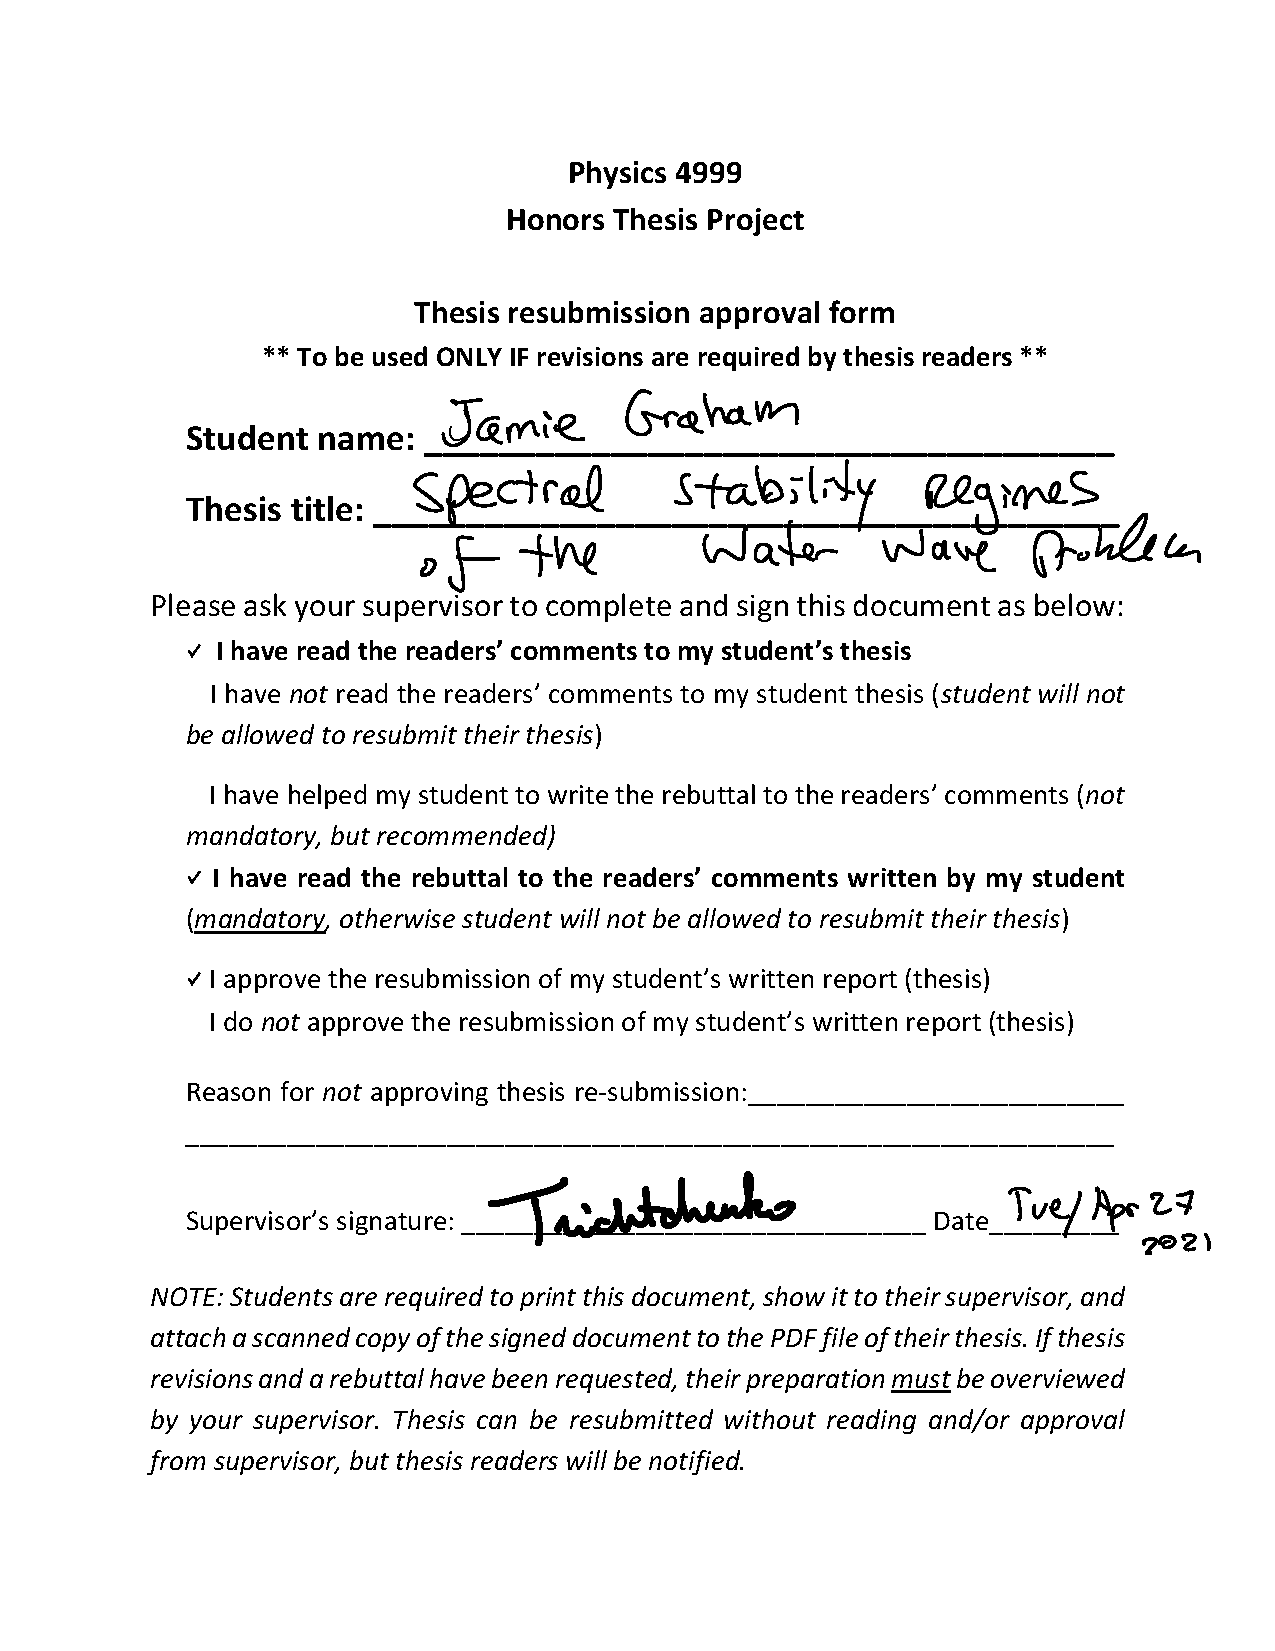
\includegraphics[scale = .9]{ResubmissionForm.pdf}
    \label{fig:my_label}
\end{figure}

\clearpage

\section{Abstract}

Dispersive Hamiltonian PDE's are an important class of problems due to their extensive applications in physics. An example of such a problem is the water wave problem, describing an incompressible, irrotational fluid using the Euler equations. Stability regimes of the full water wave problem have yet to be fully classified, with regimes determined only for certain solutions with certain parameters [\ref{olga1}]. We sought to fully classify the linear stability regime for travelling wave solutions to the general water wave problem, that is, either waves moving under an elastic boundary such as ice with surface-flexural rigidity D, or capillary-gravity waves with surface tension \(\sigma\). For this analysis, we generalized the approach by Trichtchenko et al. for identifying stability regimes of dispersive Hamiltonian PDE’s [\ref{reduced}]. We found that instabilities are governed by the choice of values for D for flexural-gravity waves, and that varying \(\sigma\) for capillary-gravity waves had no effect on these high-frequency instabilities. Various regimes of stability were found in two ice thickness ranges (cm vs mm), including a bifurcation in the centimetre range, as well as regimes of total stability and instability in the millimeter range with resonance effects that may contribute to some of the instabilities. Potential extensions of this research include a generalization of the model to waves propagating in dimensions greater than 1D, as well as the numerical computation of travelling wave solutions to investigate changes in amplitude in various stability regimes. 


\clearpage 


\section{Introduction}



\subsection{Motivation}

The mathematical basis for the modelling of a dynamical system in physics can be reduced to the solutions of partial differential equations (PDE’s) that govern the dynamics of the system. Concerning solutions of a PDE, the notion of stability describes the degree to which small perturbations of initial conditions to solutions of a given PDE generate small changes in the perturbed solution trajectories. If small perturbations of initial conditions to solutions of a given PDE generate large changes in the perturbed solution trajectories, then the PDE solution is said to be unstable [\ref{stabilitypde}]. Stability theory is a section of mathematics concerning dynamical systems that has major applications in analyzing the stability of solutions for physics-based PDE models of water wave phenomena. \\

Stability theory is integral to the study of differential equations and dynamical systems, and is a fast growing area of research from both pure and applied mathematical perspectives. The evaluation of stability regimes for various classes of PDE’s is integral to characterizing the accuracy and physical significance of solutions in space and time. Stability regimes for model equations for water waves have yet to be completely characterized, and such characterizations will also inform us about the kind of water wave phenomena that can physically exist in the real world, as well as providing useful information about water wave models for both the field of physics and environmental applied science. With the rise of global warming, weather conditions have become increasingly volatile around the world, and the accuracy of models in the field of hydrodynamic forecasting can greatly benefit from a complete mathematical characterization of stability of water waves. While unstable wave solutions are less likely to be observed in the real world, they tend to grow without bound, and thus can break the ice surface at critical amplitudes. This amplitude spiking can be observed below in Figure (\ref{wilton2}). Through restricting our research to the stability regimes of a specific class of water wave equations, we seek to further the knowledge of the field with a characterization of stability for transitional water surface flexural-gravity and capillary-gravity waves. These waves can be visualized below in Figure (\ref{icewaves}). \\

\begin{figure}[hbt!] 
\centering
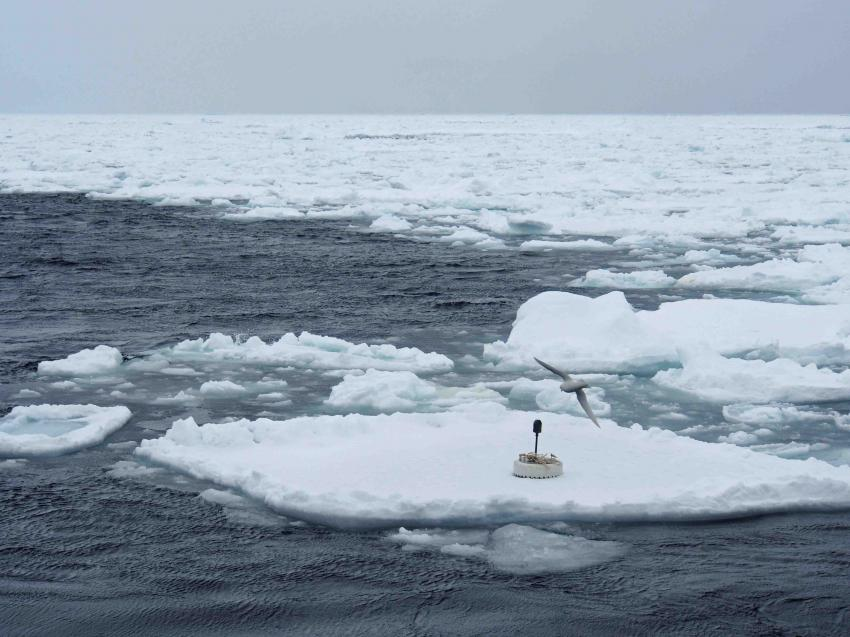
\includegraphics[scale = .4]{icewaves.jpg}
\caption{ \emph{Water waves propagating under a sheet of ice [\ref{icewavespic}]. These waves are denoted flexural-gravity waves, where the term `flexural' denotes waves which deform the structure of the fluid transversely as they propagate. In the regions where no ice is present, there exists capillary-gravity waves, where the term `capillary' denotes waves propagating at the interface of water and air where the forces of buoyancy and gravity act to maintain equilibrium.
 }}\label{icewaves}
\end{figure}

\begin{figure}[hbt!]
\centering
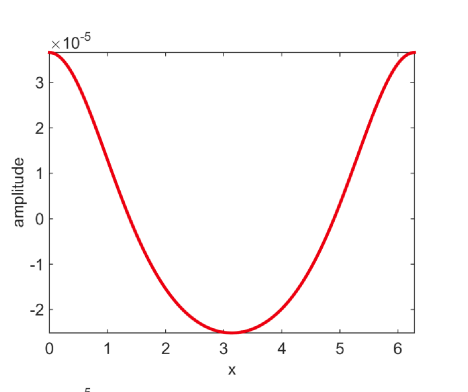
\includegraphics[width=.5\textwidth]{Profile1.png}\hfill
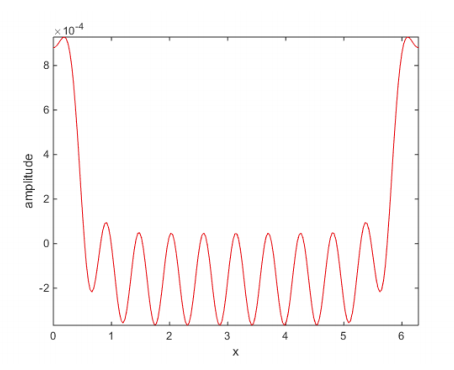
\includegraphics[width=.5\textwidth]{Profile2.png}\hfill
\caption{\emph{Amplitudes of shallow water (\(\frac{h}{\lambda} \leq 0.05\)) periodic surface flexural-gravity waves perturbed at resonant mode K = 10. The figure on the top describes a stable wave profile (\(t = 0\)), whereas the figure on the bottom describes a stable profile depicting a large amplitude resonant solution [\ref{olga1}]. }}
\label{profile}
\end{figure}

\begin{figure}[hbt!]
\centering
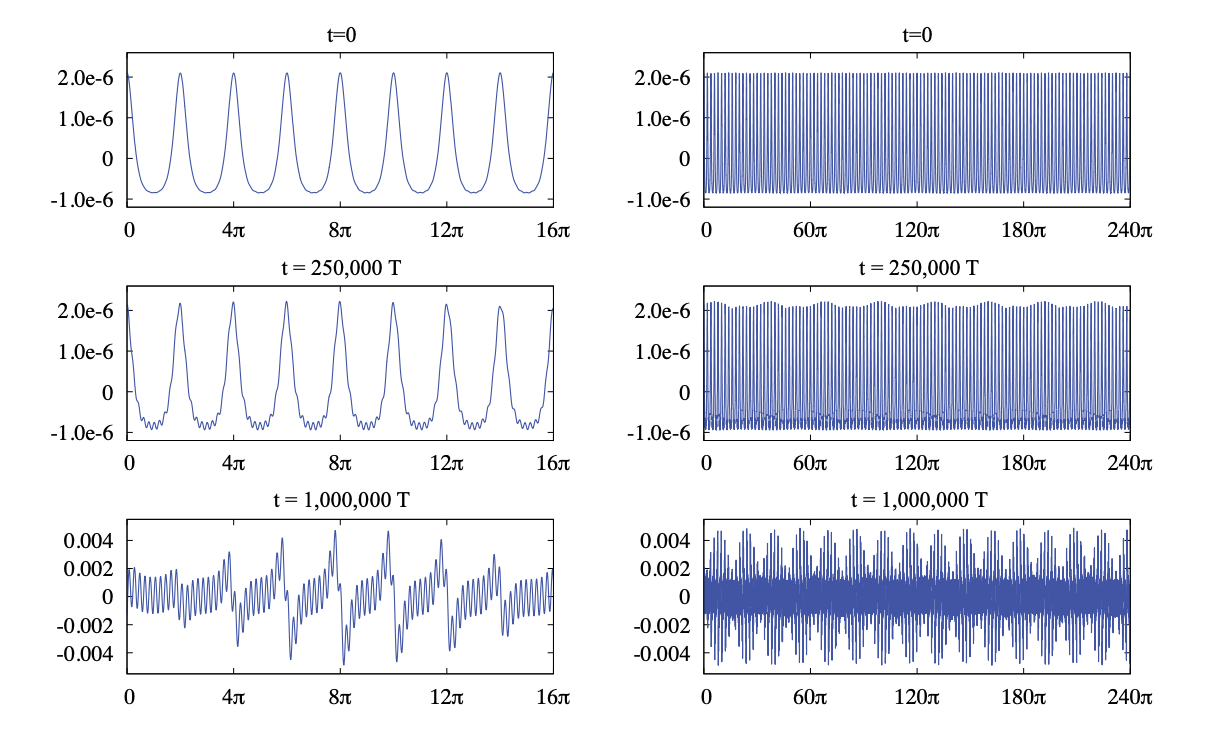
\includegraphics[width=.8\textwidth]{Wilton.png}
\caption{\emph{Wave profiles of a perturbed resonant-regime water wave solution at three different instances of time. The three profiles in succession illustrate the time evolution of the wave profile as the solution goes from a stable regime to an unstable regime with increasing t. The right column shows a macroscopic view of the wave profiles over a much larger set of periods than the left column. Note the constant maximum and minimum amplitudes of the solution at \(t = 0\), and the increasing variation of the amplitudes throughout time in the \(t = 250,000T\) and \(t = 1,000,000T\) figures. Here, T = 28.096s corresponds to the time for the underlying travelling wave solution to surpass its own wavelength [\ref{wilton}]. Note that as the system evolves, the original wave profile is completely destroyed, with a much larger amplitude that grows exponentially with time, demonstrating instability. [\ref{wilton}]}}
\label{wilton2}
\end{figure}





 As far as the terms and scope of the study, we seek to investigate the stability of small amplitude plane wave solutions to a set of partial differential equations describing the dynamics of periodic capillary-gravity waves and flexural-gravity waves under ice. We study the effects of a high-frequency perturbation of the system, which has previously been found to yield unstable regimes for particular solutions to the water wave problem [\ref{wilton2}]. These unstable regimes are referred to as high-frequency instabilities in the literature.  Upon investigating various regimes of the system by varying the physical parameters of our equation of motion, we seek to understand the stability regimes in both the centimetre and millimetre ice thickness ranges. \\
 

 We restrict our focus to that of scalar, dispersive Hamiltonian PDE’s of order 2N+1, \(N \epsilon \mathbb{N}^{+}\) with one spatial and time dimension for simplicity. The constraint of a Hamiltonian system necessitates conservation of energy, whereas the odd order constraint necessitates the dispersiveness of the system, that is, the lack of even, dissipative terms. Due to the lack of such terms, dispersive systems are generally more difficult to characterize the stability of, thereby providing a rationale for focusing on the aforementioned class of equations. \\
 
 
 \subsection{Background and Objectives}
 
  In this section, we seek to present a set of conditions on our system such that we can determine stability of wave solutions. A physical description of our system is given below in Figure (\ref{wavesindeed}). In the Eulerian picture, the solution of this system amounts to determining the fluid velocity vector field \(u(x,z,t)\) that evolves in time and space according to Euler's incompressible equations, employing the appropriate boundary conditions. 
  
  
  \subsubsection{Equations of Motion, Boundary Conditions, and Dispersion Relation}
  
  
  Firstly, a general form of Euler's equations which express conservation of mass and conservation of momentum are, respectively:
  
  \begin{equation} \label{mass}
  \nabla \cdot u = 0  \\
\end{equation}

\begin{equation} \label{eq1}
  \frac{D u}{D t} = -\frac{1}{\rho}\nabla p 
  -g \hat{\boldsymbol{z}}  \\
  \end{equation}

Where \(\frac{D u}{D t}\) denotes the advective derivative, which represents the time rate of change of the velocity field at the moving location of the field, and p denotes pressure. Furthermore, \(\rho = 1000 \frac{kg}{m^3}\) is the density of the fluid and \(g = 9.8 \frac{m}{s^2}\) denotes gravity. We assume our fluid is ideal, meaning that it is incompressible, not subject to viscous forces, and has constant density. Physical water waves can be approximated as ideal due to the negligible effects of these assumptions. We also assume that our fluid is irrotational, and thus the vorticity of the fluid vanishes. The vorticity \( \omega \) of our fluid is defined as: 


 
 \begin{equation} \label{eqn3}
  \omega = \nabla \times u = 0  \\
\end{equation}
  
This implies \(u\) is a conservative vector field, and thus there exists a potential function \(\phi\) such that \( u = \nabla \phi\). Physically, this \(\phi\) is the velocity potential of our fluid. Substituting this into (\ref{mass}), we recover Laplace's equation:

 \begin{equation} \label{laplace}
  \nabla^2 \phi = 0  \\
\end{equation}
 
Adopting the potential formalism, a complete characterization of the trajectories of our system can be reduced to solving for this potential function \(\phi(x,z,t)\). Let us now consider the thin plate equation which forms the basis for our modelling of the sheet of ice on the surface of the water. The pressure can be expressed as:

\begin{figure}[hbt!] 
\centering
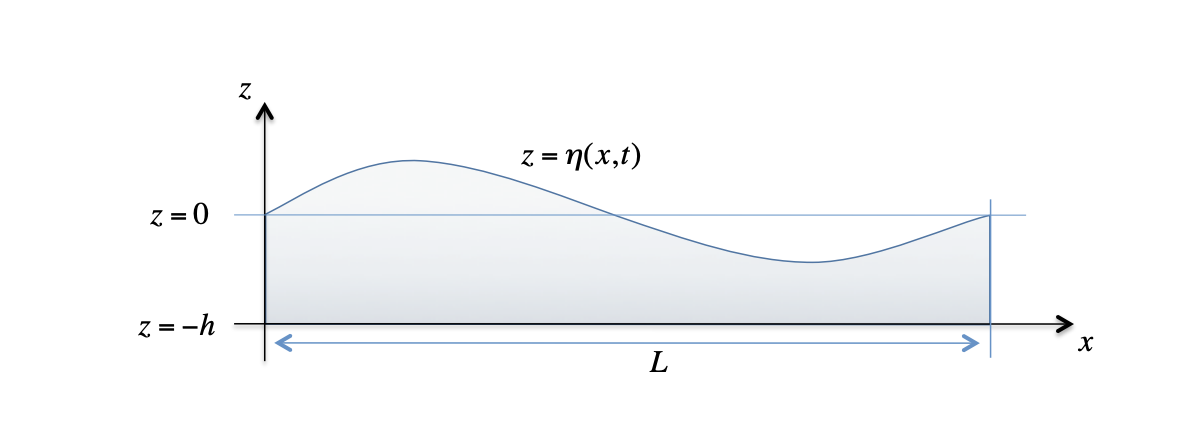
\includegraphics[scale = .9]{WaterPicture.png}
\caption{ \emph{Water waves incident on a thin elastic ice sheet that deforms with the surface of the water. Fluid domain is in the x-z plane and spans \(z=\eta(x,t)\) to \(z=-h\) [\ref{reduced}].}}\label{wavesindeed}
\end{figure}
  

 
\begin{equation} \label{elastic}
  \hspace{-20} D \nabla^4 \eta + \sigma \nabla^2 \eta + \rho_{e} h \frac{\partial \eta^2}{\partial t^2} = p \\
\end{equation}

Where \(\nabla\) is the two dimensional del operator acting in the (x,y) plane, \(\eta\) is the wave profile, \(\rho_e\) is the ice density, p denotes pressure, \(\sigma\) denotes surface tension, and \(D\) denotes surface flexural-rigidity of ice [\ref{bandstructure}]. \(D\) is a structural parameter of the ice that describes the intrinsic resistance to deformation, or rigidity of the ice. It can be expressed as: 
 
\begin{equation} \label{rigidity}
  D = \frac{Ed^3}{12(1-\nu^2)} \\
\end{equation}
 \\
 
 Here \(E\) is the Young's Modulus of our elastic boundary (ice), which represents the material `stiffness' of our elastic boundary. The parameter d is the thickness of the ice, and \(\nu\) is the Poisson's ratio of ice, which is a measure of the deformation of a material perpendicular to the direction of loading forces on the elastic boundary. In comparison to \((\ref{elastic})\), the pressure at the interface between the water and the ice sheet can also be expressed as: 

\begin{equation} \label{press}
p = -\rho \frac{\partial \phi}{\partial  t}_{z=0} - \rho g \eta \\
\end{equation}

\vspace{10}

Where \(\rho\) denotes the density of water. 
Let us now consider the boundary conditions of our system. The dynamic boundary condition on the surface of the water follows from conservation of momentum, and can be written as follows: 

 \begin{equation} \label{dyn}
  \hspace{100} \phi_{t} + \frac{1}{2} \lvert \nabla \phi \rvert^2 + g \eta = -\frac{p}{\rho}   \hspace{30} (z = \eta(x,t)) \\
\end{equation}

\vspace{10}

The kinematic boundary condition at the surface ensures that a particle on the surface remains on the surface as time evolves in the system. It can be derived in the potential formulation by taking the total derivative of the distance function \(P(x,z,t) = z - \eta(x,t)\). The kinematic boundary condition is:


\begin{equation} \label{kin}
 \hspace{100}\partial_t \eta  + \phi_{x}\eta_{x} = \partial_z \phi \hspace{57}    (z = \eta(x,t))\\
\end{equation}


The final boundary condition to consider is the impermeable bed condition, namely that the z derivative of the velocity potential \(\phi\) is zero at \(z = -h\), which can be considered physically as the bottom of the fluid domain. The bed condition is:

\begin{equation} \label{bed}
 \hspace{100} \partial_z \phi   = 0 \hspace{95}    (z = -h)\\
\end{equation}


We have now defined all the relevant equations in our system. Restricting our analysis to the linear regime and combining (\ref{laplace}), (\ref{elastic}), (\ref{press}), (\ref{dyn}), (\ref{kin}), and (\ref{bed}), we can write our linearized equations of motion as:

 \begin{align} \label{phieq}
    \phi_{t} + g\eta = \frac{1}{\rho}( -D\eta_{4x} - \sigma_{2x} ) \\ \label{etaeq}
    \partial_t \eta  = \partial_z \phi  
 \end{align}
 
Note that these two equations can be combined by taking the time derivative of (\ref{phieq}) and plugging in (\ref{etaeq}), using the commutative property of partial derivatives to eliminate \(\eta\) from the system. Upon doing this, we recover:

\begin{equation} \label{phieq2}
 \phi_{tt} + g\phi_{z} = -\frac{D\phi_{(4x)z}}{\rho} - \frac{\sigma\phi_{(2x)z}}{\rho} \\
\end{equation}
 
\vspace{10} 
 
We will now plug in a small-amplitude solution \(\phi = \epsilon e^{i(kx-\omega t)}\cosh{(k(h+z))} \) into (\ref{phieq}) in order to determine the dispersion relation, and thus the wave speed of our solution. Plugging in this solution, the dispersion relation can be derived: 

\vspace{-20} 

\begin{align}

 \centering{
 -\omega^2 + gk\tanh(kh) = \frac{-Dk^5\tanh(kh)}{\rho} + \frac{\sigma k^3 \tanh(kh)}{\rho}
 
 \\ \vspace{15} \hspace{-500} \implies

 \vspace{15} 
 
 \omega^2 = (gk - \frac{\sigma k^3}{\rho} + \frac{D k^5}{\rho})\tanh{(kh)} 
 }
 \\ 
\end{align}
\vspace{-40}

Taking the square root

\vspace{10}

\begin{equation} \label{dispersion}
 \omega = \sqrt{(gk - \frac{\sigma k^3}{\rho} + \frac{D k^5}{\rho})\tanh{(kh)}}  
 \\
\end{equation}

Using the familiar expression relating wave speed to dispersion \(\omega = ck\):

\begin{equation} \label{V}
 ck = \sqrt{(gk - \frac{\sigma k^3}{\rho} + \frac{D k^5}{\rho})\tanh{(kh)}}
 \\
\end{equation}

Assuming that the solution we are linearizing about is \(2 \pi\) periodic, we can set \(k = 1\) and then solve for the wave speed. Let us define the wave speed, \(V_{0}\) as:

\begin{equation} \label{V}
 V_{0} = \sqrt{(g - \frac{\sigma }{\rho} + \frac{D }{\rho})\tanh{(h)}}  
 \\
\end{equation}

It is important to note that physically, either \(D = 0\) and there is no elastic boundary (ice), or \(\sigma = 0\) and there exists an elastic boundary. Both \(\sigma\) and D are kept in our model for completeness, but upon carrying out numerical calculations, at least one will always be set to zero in order for our results to have physical relevance.\\

Varying the surface flexural rigidity D, there should exist modes K of our travelling waves such that  resonance occurs. The resonance condition for a given mode K of these waves \(K \neq 1\) is:

\begin{equation} \label{resonance}
(g + \frac{D}{\rho})K\tanh{(h)} - (g + \frac{DK^4}{\rho})\tanh{(Kh)} = 0 
 \\
\end{equation}

This can also be done with the surface tension \(\sigma\), and the analogous resonance condition is:

\begin{equation} \label{resonancesigma}
(g - \frac{\sigma}{\rho})K\tanh{(h)} - (g - \frac{\sigma K^2}{\rho})\tanh{(Kh)} = 0 
 \\
\end{equation}

In the most general form for the water wave problem, the resonance condition can thus be written [\ref{wilton}]

\begin{equation} \label{resonancegen}
(g - \frac{\sigma}{\rho} + \frac{D}{\rho})K\tanh{(h)} - (g - \frac{\sigma K^2}{\rho} + \frac{DK^4}{\rho})\tanh{(Kh)} = 0 
 \\
\end{equation}


We will now employ a change of variables on the surface of the water \(q(x,t) = \phi(x,\eta(x,t),t) \) to combine the two equations of motion above into a single, first order equation. It can be shown [\ref{katie}] that upon implementing this change of variables, the two equations reduce to the form:\\

\begin{equation} \label{no}
q_{t} + g\eta = -\frac{1}{\rho}p
\end{equation}

\intertext{\flushleft{which for our problem yields}}

\begin{equation} \label{local}
q_{t} + g\eta = \frac{1}{\rho}( -D\eta_{4x} - \sigma_{2x} )
\end{equation}

\intertext{\flushleft{which we will refer to from now on as the local equation.}}
\vspace{10}

We now approach our stability problem from a slightly different perspective and look to the Ablowitz, Fokas, and Musslimani (AFM) formulation [\ref{AFM}] for the non-local behaviour of the system. The non-local equation of motion is derived by rewriting Laplace's equation for the bulk fluid using only surface variables, namely \(\eta\) rather than q [\ref{katie}]. It can be written as:


\begin{equation} \label{no}
\int_{0}^{L} e^{-ikx}(\eta_{t}\cosh(k(h+\eta)) - iq_{x}\sinh(k(h+\eta))) = 0
\end{equation}

Upon considering strictly the linear regime and expanding the hyperbolic sinusoids using the sum trigonometric identities:

\begin{equation} \label{no} 
\cosh(x+y) = \cosh(x)\cosh(y) + \sinh(x)\sinh(y) 
\end{equation}

\begin{equation} \label{no}
\sinh(x+y) = \sinh(x)\cosh(y) + \sinh(y)\cosh(x) 
\end{equation}

\intertext{we recover for our system}

\begin{equation} \label{non-local}
\int_{0}^{L} e^{-ikx}(\eta_{t} - iq_{x}\tanh(kh)) = 0
\end{equation}

\vspace{10}

This equation (\ref{non-local}) will be referred to from now on as the non-local equation in the AFM formulation. \\
\vspace{5}

\subsubsection{The Spectral Stability Problem}

We will now discuss some properties of the spectral stability problem, which we are concerned with in determining the stability regimes of our system. The spectral stability problem in functional analysis is a generalization of the eigenvector-eigenvalue problem to infinite dimensional function spaces. We will use first order perturbation theory in our stability analysis, and so in the context of our system, the eigenfunctions of our spectral stability problem will be the first order perturbations of our velocity potential q and wave profile \(\eta\) at the surface of the water. Letting \(w = (q,\eta)\), a general spectral stability problem can be written as:\\


\begin{equation} \label{specstab}
 \mathscr{L}w = \lambda w
\end{equation}

Where \(\mathscr{L}\) is a linear differential operator, \(w\) is a vector of eigenfunctions q and \(\eta\) of the problem, and \(\lambda\) is an eigenvalue of the problem. Since the problem is infinite dimensional, the set of eigenvalues spans a continuous range of values is thus denoted the \emph{spectrum}. The spectral problem admits a Fourier decomposition solution for the eigenfunctions of the problem. \\

\vspace{15} 

Floquet's theorem tells us that all bounded solutions of the spectral problem (12) are of the form: 

\begin{equation} \label{floquet}
  w(x,t) = e^{i\mu x} \sum_{m=-\infty}^{\infty} \hat\mu^{(1)}_m e^{imx} + c.c
\end{equation}

Where the Floquet parameter \(\mu\) governs the period of the perturbation \((T = \frac{2 V_0\pi}{\mu})\), and m is the mode of a given eigenvalue in the spectrum, and c.c denotes the complex conjugate. Plane waves in the Fourier decomposition corresponding with a given Fourier mode m have an associated eigenvalue corresponding with the Fourier mode m.  Substituting this solution into the spectral problem (\ref{specstab}) yields an expression for eigenvalues as a function of \(\mu +\)m. Therefore, we have:

\begin{equation} \label{eq1}
  \mathscr{L}w(m+\mu) =   \lambda(m+\mu) w(m+\mu)
\end{equation}

A solution to a PDE is considered spectrally stable if the full spectrum of eigenvalues for the spectral problem lie in the closed left half of the complex plane. Equivalently, the solution is spectrally stable if all eigenvalues are either pure imaginary, or have negative real part. This is a generalization of the standard notion of stability of systems of differential equations about equilibria, where negative eigenvalues of the linearized system tend to describe stable sinks, and positive ones describe unstable sources.\\

We seek to classify the stability regimes—that is—the spectral stability of the aforementioned small-amplitude solutions to our equations in various parameter regimes, varying parameters such as the surface flexural rigidity \(D\), the surface tension between air and water \(\sigma\), as well as the water depth h. \\



In terms of the scope of the study, we seek to exploit properties of our system that yield necessary conditions for instability of solutions, namely the collisions of eigenvalues of the spectral stability problem, and also the Krein signature condition of these eigenvalues. We will describe these conditions below. As previously mentioned, if all the eigenvalues of the spectral problem have negative or zero real part, then the solutions are stable. However, if eigenvalues have positive real part, then the solutions can be unstable.\\



Usually, if there exists eigenvalues of a stability problem with non-zero positive real part, then such a dynamical system is unstable. For our system, if there exists eigenvalues with negative non-zero real part, then there must exist eigenvalues with positive non-zero real part as well in the spectral stability problem. This is a result of the necessity that our system is Hamiltonian. Thus, simply the presence of eigenvalues with non-zero real part is enough to determine the possible instability of the system. Note that under our perturbation, the spectrum of eigenvalues depends continuously on the amplitude of our solution \(q(x,t)\). As the amplitude increases with time, eigenvalues of the spectral problem can diverge from the pure imaginary axis into the real part of the complex plane. In order for this to happen, eigenvalues of different modes on the pure imaginary axis must collide first. If a collision occurs and the eigenvalues spread out into the real part of the complex plane, by the symmetry of the Hamiltonian system, the eigenvalues must come in complex conjugate pairs, as well as pairs reflected across the imaginary axis, so that the Hamiltonian preserves realness, and thus at least one of such eigenvalues would have positive real part, implying instability [\ref{reduced}]. This would not be possible if it weren't for the initial collision of the eigenvalues of two different modes. Therefore, another necessary condition for instability is the collision of eigenvalues of the spectral stability problem. Cases of such collisions can be observed in Figure (\ref{eigenvaluesgraph}). \\



\begin{figure}[htp]
\centering
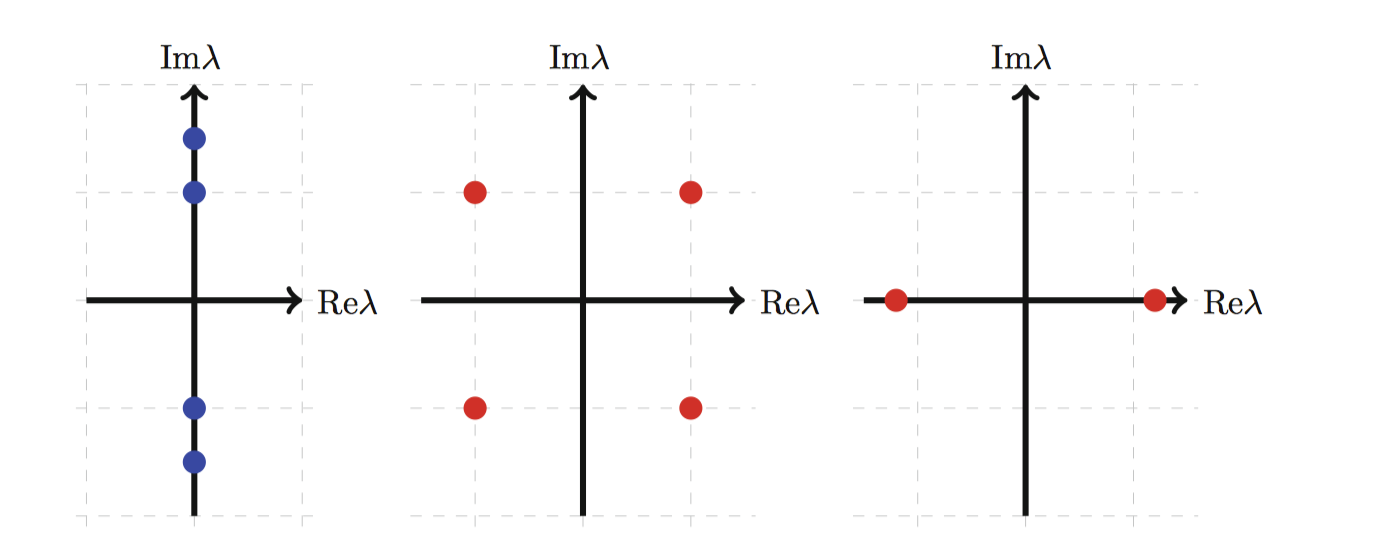
\includegraphics[scale = 0.7]{Eigenvalues.png}
\caption{\emph{Three different configurations of the smallest number of eigenvalues \(\lambda\) of the spectral stability problem of a Hamiltonian system, showing the symmetry about the real and imaginary axes. On the left (in blue), is the stable regime. The centre and right panel are the unstable regimes (in red).}}\label{eigenvaluesgraph}

\end{figure}

\\

The collision condition for two eigenvalues of modes m and l can be written as:


 \begin{equation} \label{eq1}
  \lambda(\mu + m) = \lambda(\mu + l)
\\
\end{equation}

In order to reduce the number of unknowns we are working with, let us set \(\mu \rightarrow \mu + m \) and \(n \rightarrow |l-m|\). From here on, this n will be referred to as the Fourier mode difference parameter. Then, our collision condition reads: 

 \begin{equation} \label{eigenvaluecollisioncondition}
  \lambda(\mu) = \lambda(\mu + n)
\\
\end{equation}

Thus, we are concerned now only with the difference (l-m) in modes of the colliding eigenvalues, rather than the actual values of l and m themselves. Secondly, in order for our Hamiltonian system to conserve energy, for different eigenvalues of modes m and l to collide, they must have opposing signatures so as to preserve the energy, that is if one contributes positively to the energy, the other one has to contribute negatively. Thus, we need a condition that lets us know that our eigenvalues of modes m and l are of opposing signature. Such a condition is called the Krein signature condition:

 \begin{equation} \label{krein1}
  s = (\mu + l)(\mu + m) < 0
\\
\end{equation}

Again, making the substitutions \(\mu \rightarrow \mu + m \) and \(n \rightarrow |l-m|\), we recover an analogous expression to (16) for our signature of colliding eigenvalues condition:

 \begin{equation} \label{krein2}
  s = (\mu)(\mu + n) < 0
\\
\end{equation}


Using these conditions (\ref{eigenvaluecollisioncondition}) and (\ref{krein2}), as well as the expression for the eigenvalues \(\lambda\), a stability function can be defined, the roots of which determine the spectral stability of the system. If the roots are purely imaginary, then the solutions are stable, but if the roots are real, then the system can have instabilities.  We seek to examine the conditions on the coefficients of the aforementioned stability function that will necessitate purely imaginary eigenvalues, and thus the spectral stability of the wave solutions. \\

\subsubsection{The Resonance Method of Ice Destruction}

Lastly, we will consider the resonant regimes of the water-wave ice system. A common procedure in the applied physical sciences in the field of hydrodynamics is called the resonance method of ice destruction. The theory behind the method is that when the magnitude of the phase velocity of a heavy load moving on the ice is close to the magnitude of the phase velocity of the flexural-gravity waves underneath, the water no longer supports the ice against gravity, the system is in resonance, and the amplitudes of the flexural-gravity waves grow exponentially such that eventually the ice breaks [\ref{resonancemethod}]. An application of this method is hovercraft `icebreaking`, used in order to clear passageways for water transportation, as demonstrated in Figure (\ref{Hovercraft}) below. Numerical values for such phase velocities are also used in the production of ice-road signs indicating speed limits for which vehicles must obey in order for the resonance method of ice destruction to not occur.
\\

\begin{figure}[hbt!]
\centering
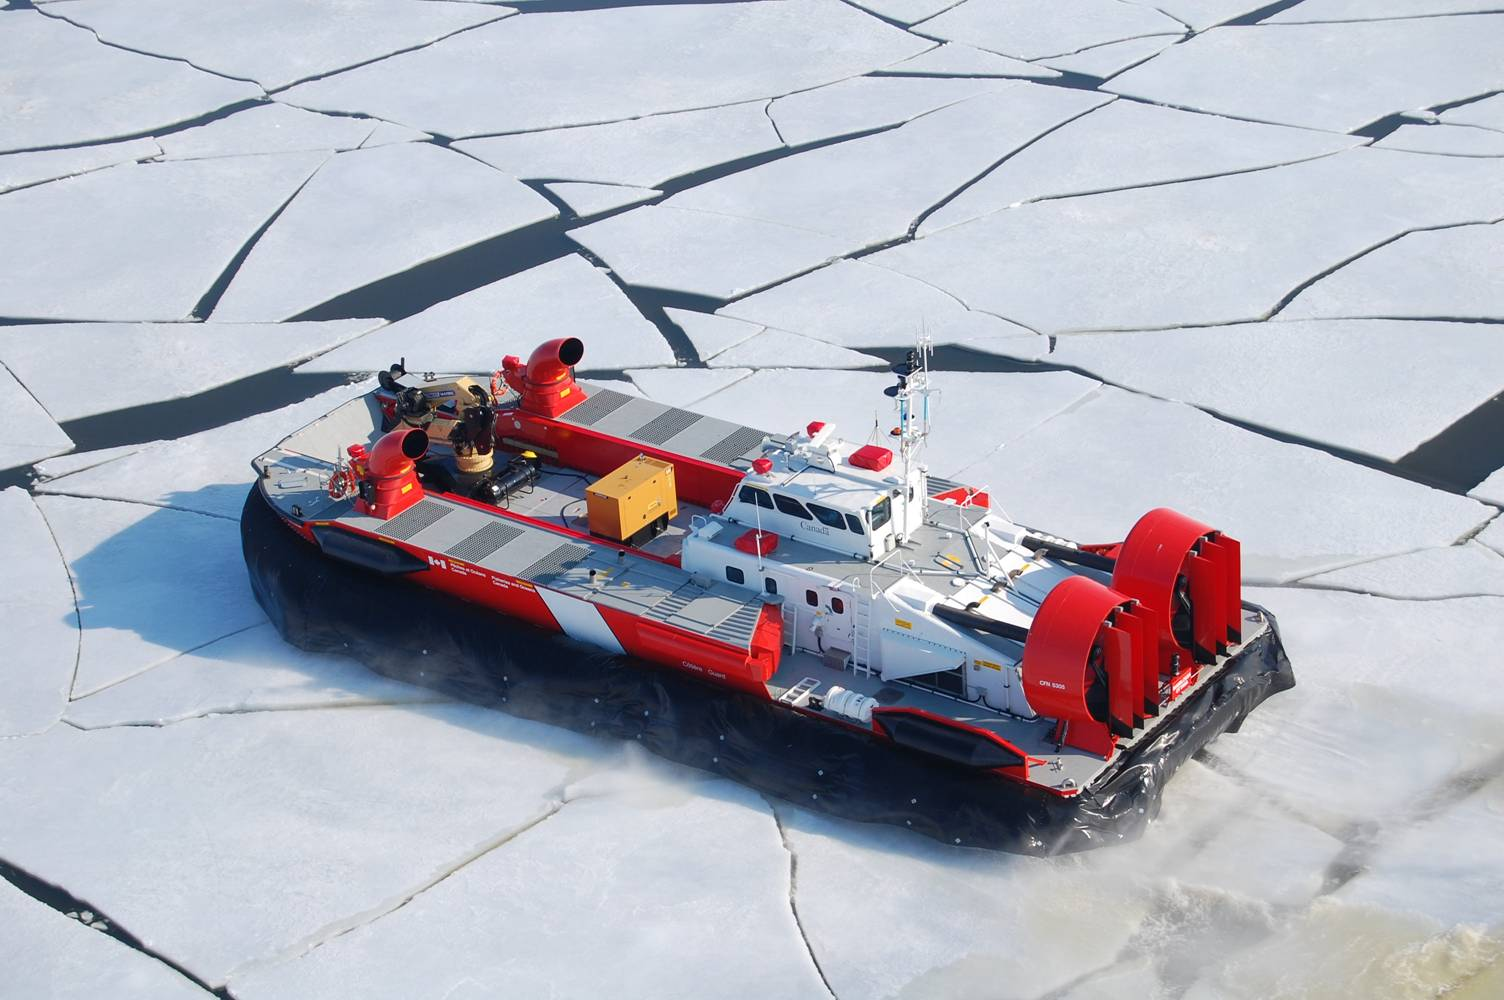
\includegraphics[scale = .4]{Hovercraft.jpg}
\caption{\emph{A hovercraft moving on ice and demonstrating the resonance method of ice destruction. The hovercraft matches the linear phase velocity of the flexural-gravity waves under the ice and induces resonance-based amplitude spikes that break the ice as they propagate. [\ref{hovercraft}]}}\label{Hovercraft}
\end{figure}

The introduction will now be followed by a literature review, a detailed description of our experimental methodology, our results and then a conclusion and discussion of the findings. 

\subsection{Literature Review}

Stability regimes have been previously determined for certain classes of particular water wave solutions, such as the standard soliton solutions of the Korteweg-de-Vries (KdV) equation [\ref{kdv}], and the solitary wave solutions of the Boussinesq equation [\ref{bouss}]. For the general water wave problem, the linear stability regime has yet to be fully characterized under the full variation of physically relevant parameters. Trichtchenko, Milewski, Parau, and Vanden-Broeck analyzed the stability of particular solutions for periodic two dimensional travelling flexural-gravity waves in deep and shallow water [\ref{olga1}]. Through solving the non-linear Schrodinger equation derived from Euler’s equations, it was found that in the regime of large surface flexural-rigidity, non-linear models tend to exhibit stable solutions, deviating from the behaviour of their linear counterparts, which exhibit high-frequency instabilities in this regime [\ref{olga1}]. Gao, Wang, and Vanden-Broeck also studied the dynamics of propagating deep water flexural-gravity waves under a floating flexible ice plate [\ref{gao}]. The surface ice exerts pressure on the water, which accounts for the non-linearity of the model. A numerical simulation of the wave solutions was computed, encapsulating the response to a localized pressure distribution moving at a rate slightly under the wave phase speed—this is known as the trans-critical regime. Symmetric, moderate-amplitude solitary wave solutions to Euler’s irrotational water wave equations with flexural-gravity boundary conditions were numerically found to have finite amplitude within this regime, and thus were determined as stable [\ref{gao}].\\ 


Presently, research has been performed attempting to characterize the stability regimes of particular solutions to the water wave problem for deep water \(\frac{h}{\lambda} \geq 0.5\), surface flexural-gravity waves [\ref{olga1},\ref{wilton},\ref{gao},\ref{cap2}]. The effect of variation in parameters such as the surface flexural-rigidity, and surface tension of particular solutions to these systems in the shallow water regime \(\frac{h}{\lambda} \leq 0.05\) has also been studied [\ref{olga1},\ref{wilton},\ref{katie},\ref{gao}] . Little attention has been paid to the transitional water regime \(0.05 \leq \frac{h}{\lambda} \leq 0.5\) and thus this regime will be a focus of this paper. Here, h is the depth of the water and \(\lambda\) is the wavelength of the propagating wave. In addition, only the stability regimes of particular solutions to the water-wave problem have been studied and thus we will attempt to resolve the linear stability regime of the full water-wave problem in general. Stability properties of general classes of water wave solutions have been studied [\ref{bryant},\ref{hammack}], but not in great detail for the aforementioned flexural-gravity and capillary-gravity waves resulting from the water-wave problem in question. In addition, little research has been conducted investigating conditions on the spectral stability functions that affect stability of wave solutions. We intend to formulate a set of necessary criteria for such functions to determine resultant wave stability. The advantages of studying the full water-wave problem in the transitional water regime lie in the scarcity of literature attempting to characterize stability regimes of this system, as well as possible environmental applications and extensions of the research. Disadvantages of the study include the lack of pre-existing efforts to quantify the aforementioned stability regimes in question--this would help as a comparative benchmark for our findings--as well as the highly non-linear dispersion relations for such equations, making our spectral stability functions difficult to compute due to the presence of hyperbolic tangents, and fifth order surface-flexural terms. We intend to mitigate the latter disadvantage by solving an eigenvalue matrix constructed from the local and non-local equations (\ref{local}) and (\ref{non-local}) in order to determine an analytical expression for the eigenvalue spectrum. The aforementioned considerations from the literature will be kept in mind to help inform the progress and completion of this study. \\

We hypothesize that our small-amplitude solutions to the water wave problem will exhibit regimes of stability and instability under high-frequency perturbations in multiple regimes of the surface flexural rigidity, surface water tension, and water depth. We also hypothesize that with increasing values of the surface flexural-rigidity D, we will see more instabilities in our system, consistent with the findings of previous research of particular solutions to the water-wave problem [\ref{olga1}]. Concerning the eigenvalues of the spectral problem, for colliding eigenvalues of different modes m and l, there should exist values for the difference between m and l such that the system can exhibit instabilities, and specific parameter regimes such that these instabilities can occur. 
\\

\section{Methodology}

 \\
 
This section details the methodology for our stability analysis. We plug first order perturbative solutions into our equations of motion (\ref{local}) and (\ref{non-local}) in order to derive a special 2x2 matrix. The eigenvalues of this matrix give us an analytical expression for the eigenvalues of the spectral stability problem as a function of the Fourier modes in the Fourier-Floquet decomposition of our first order perturbation. From there, a set of stability functions can be defined using this eigenvalue function, as well as the instability criteria  (\ref{eigenvaluecollisioncondition}) and (\ref{krein2}). The roots of these stability functions determine the stability of our system in a given parameter regime. These stability functions depend on constant parameters D, \(\sigma\), h, and n. We hypothesize that these parameters can be varied to alter the stability of the system, which we can determine numerically by determining the existence of real roots in the Krein interval defined below (\ref{interval2}) for a fixed set of the above parameters. 
 
\subsection{First Order Perturbations of The Non-Local Equation}

For our stability analysis for the water wave-ice problem, we start from the equations of motion which are, respectively:

\begin{align} \label{system}
q_{t} + g\eta = \frac{1}{\rho}( -D\eta_{4x} - \sigma_{2x} )\\\label{system2}
\int_{0}^{L} e^{-ikx}(\eta_{t} - iq_{x}\tanh(kh)) = 0
\end{align}


Let us start with the non-local equation (\ref{system2}). We now implement first-order perturbation theory on our solutions q and \(\eta\). The zero'th order perturbation terms drop out of our system and we are left with the first order terms, which can be expressed via Floquet theory (\ref{floquet}). The first-order perturbations for q and \(\eta\) can be written as

\begin{equation} \label{q}
  q^{(1)}(x,t) = \delta_{0}e^{\lambda t}\sum_{m=-\infty}^{\infty}b_{m}e^{i(m+\mu)(x-V_{0}t)}
\\
\end{equation}


\begin{equation} \label{eta}
  \eta^{(1)}(x,t) = \delta_{0}e^{\lambda t}\sum_{m=-\infty}^{\infty}a_{m}e^{i(m+\mu)(x-V_{0}t)}
\\
\end{equation}

We now seek to determine an analytical result for our spectral stability eigenvalue function by setting up a 2x2 matrix for this system and solving for the eigenvalues \(\lambda\). We shall now derive the expression that will constitute the first row of this matrix. Plugging (\ref{q}) and (\ref{eta}) into the non-local equation (\ref{system2}), we recover the expression:

\begin{align}

    \int_{0}^{L} e^{-ikx}((\lambda - i(m+\mu)V_{0}\delta_{0}e^{\lambda t}\sum_{m=0}^{\infty}a_{m}e^{i(m+\mu)(x-V_{0}t)} \hspace{2} - \hspace{3}  i(i(m+\mu)\delta_{0}e^{\lambda t}\sum_{m=0}^{\infty}b_{m}e^{i(m+\mu)(x-V_{0}t)}\tanh(kh))dx = 0
    
    \\ \vspace{15} \implies

    \vspace{15}
    \int_{0}^{L} e^{-ikx}((\lambda - i(m+\mu)V_{0}\delta_{0}e^{\lambda t}\sum_{m=0}^{\infty}a_{m}e^{i(m+\mu)(x-V_{0}t)} \hspace{2} + (m+\mu)\delta_{0}e^{\lambda t}\tanh(kh)\sum_{m=0}^{\infty}b_{m}e^{i(m+\mu)(x-V_{0}t)}dx = 0
    
    \\ \vspace{15} \implies

    \vspace{15}
    \centering
    \int_{0}^{L} e^{\lambda - iV_{0}t}\sum_{m=0}^{\infty}[(\lambda - i(m+\mu)V_{0})\delta_{0}a_{m} + \tanh(kh)(m+\mu)\delta_{0}b_{m} ] e^{i(m+\mu-k)x} = 0     
    
    \\ \vspace{15} \flushleft{assuming our perturbative solutions are well-behaved, we can interchange the sum and integral and evaluate the plane wave integral as follows:}
    
    \vspace{15}
    \centering{
    e^{\lambda - iV_{0}t}\sum_{m=0}^{\infty}[(\lambda - i(m+\mu)V_{0})\delta_{0}a_{m} + \tanh(kh)(m+\mu)\delta_{0}b_{m} ] \frac{e^{i(m+\mu-k)x}}{i(m+\mu-k)}\Big|_0^L + C = 0 }    
    \\ \vspace{15} 
    
    \flushleft{without loss of generality we can set C = 0 and then evaluate this expression at the upper/lower limits of the integral:}
    
    \vspace{15}
    \centering{
    e^{\lambda - iV_{0}t}\sum_{m=0}^{\infty}[(\lambda - i(m+\mu)V_{0})\delta_{0}a_{m} + \tanh(kh)(m+\mu)\delta_{0}b_{m} ] \frac{e^{i(m+\mu-k)L} - 1}{i(m+\mu-k)} = 0 }  
    
    \\ \vspace{15} \flushleft{In attempts to simplify this expression slightly, we factor \(e^{i(m+\mu+k)\frac{L}{2}}\) out of the expression:}
    
    \vspace{15}
    \centering{
    e^{\lambda - iV_{0}t}\sum_{m=0}^{\infty}[(\lambda - i(m+\mu)V_{0})\delta_{0}a_{m} + \tanh(kh)(m+\mu)\delta_{0}b_{m} ]e^{i(m+\mu-k)\frac{L}{2}}[\frac{e^{i(m+\mu-k)\frac{L}{2}} - e^{-i(m+\mu-k)\frac{L}{2}}}{i(m+\mu-k)}] = 0 }  
    
    \\ \vspace{15} \flushleft{recognizing that  \(\sin((m + \mu + k)\frac{L}{2}) = \frac{e^{i(m+\mu-k)\frac{L}{2}} - e^{-i(m+\mu-k)\frac{L}{2}}}{2i}\), we can rewrite the above expression as:}
    
    \vspace{15}
    \centering{
    e^{\lambda - iV_{0}t}\sum_{m=0}^{\infty}[(\lambda - i(m+\mu)V_{0})\delta_{0}a_{m} + \tanh(kh)(m+\mu)\delta_{0}b_{m} ]e^{i(m+\mu-k)\frac{L}{2}}[\frac{2\sin((m + \mu - k)\frac{L}{2})}{(m+\mu-k)}] = 0 }  
    
    \vspace{15} \flushleft{Using the orthogonality of the plane wave basis, we can recognize that under an inner product with the basis function from the n'th Fourier mode:}
    
    \vspace{15}
    \centering{\int_{0}^{L} e^{\lambda - iV_{0}t}\sum_{m=0}^{\infty}[(\lambda - i(m+\mu)V_{0})\delta_{0}a_{m} + \tanh(kh)(m+\mu)\delta_{0}b_{m} ]\frac{2\sin((m + \mu - k)\frac{L}{2})}{(m+\mu-k)}[e^{i(m+\mu-k)\frac{L}{2}}e^{i(n+\mu-k)\frac{L}{2}}]dx = 0}  
    
    \\ \vspace{15} \flushleft{The inner product collapses the sum in this expression since all terms vanish other than the case where \(n = m\)}
    
    \vspace{15}
    \centering{
    \int_{0}^{L} e^{\lambda - iV_{0}t}[(\lambda - i(m+\mu)V_{0})\delta_{0}a_{m} + \tanh(kh)(m+\mu)\delta_{0}b_{m} ]\frac{2\sin((m + \mu - k)\frac{L}{2})}{(m+\mu-k)}[e^{i(m+\mu-k)L}]dx = 0 } 
    
    \\ \vspace{15} \flushleft{Upon evaluation of this integral, we recover:}
    
    \vspace{15}
    \centering{
    e^{\lambda - iV_{0}t}[(\lambda - i(m+\mu)V_{0})\delta_{0}a_{m} + \tanh(kh)(m+\mu)\delta_{0}b_{m} ]\frac{2\sin((m + \mu - k)\frac{L}{2})}{(m+\mu-k)}e^{i(m+\mu-k)L}L = 0 } 
\end{align}

\vspace{-20}

Since this equation is equal to 0 we can divide constant terms out on the left-hand-side to obtain the first row of the matrix:

\vspace{15} 

\begin{equation} \label{matrixrow1}
   [(\lambda - i(m+\mu)V_{0})a_{m} + \tanh(kh)(m+\mu)b_{m} ] = 0 
\\
\end{equation}

\vspace{15}

\subsection{First Order Perturbations of The Local Equation}

\vspace{15}

Now, we look to the local equation (\ref{system}) and we plug in the first order perturbations (\ref{q}) and (\ref{eta}). In doing so, we derive the second row of the stability eigenvalue matrix we seek.

\vspace{-10} 

\begin{align}

 \centering{
 \sum_{m = 0}^{\infty} \bigg[(g\delta_{0} + \frac{D\delta_{0}(m+\mu)^4}{\rho} - \frac{\sigma \delta_{0} (m+\mu)^2}{\rho})a_{m} - (\lambda - i(m+\mu)V_{0})\delta_{0}b_{m}\bigg]e^{i(m+\mu-k)x} = 0 
 }
    
 \vspace{15} \flushleft{{Using the orthogonality of the plane wave basis, we can recognize that under an inner product with the basis function from the n'th Fourier mode:}}
 
 \vspace{15}
 \centering{
 \int_{0}^{L} \sum_{m = 0}^{\infty} \bigg[(g\delta_{0} + \frac{D\delta_{0}(m+\mu)^4}{\rho} - \frac{\sigma \delta_{0} (m+\mu)^2}{\rho})a_{m} - (\lambda - i(m+\mu)V_{0})\delta_{0}b_{m}\bigg]e^{i(m+\mu-k)x}e^{i(n+\mu-k)x} = 0 }

\vspace{15} \flushleft{Again, the inner product collapses the sum in this expression since all terms vanish other than the case where \(n = m\)}
 
 \vspace{15}
 
 \centering{
 \int_{0}^{L}\bigg[(g\delta_{0} + \frac{D\delta_{0}(m+\mu)^4}{\rho} - \frac{\sigma \delta_{0} (m+\mu)^2}{\rho})a_{m} - (\lambda - i(m+\mu)V_{0})\delta_{0}b_{m}\bigg]e^{2i(m+\mu-k)x} = 0 
 }
 
 \vspace{15} \flushleft{Evaluating this integral and plugging in the bounds, we get:}
 
 \vspace{15}
 
 \centering{
 \bigg[(g\delta_{0} + \frac{D\delta_{0}(m+\mu)^4}{\rho} - \frac{\sigma \delta_{0} (m+\mu)^2}{\rho})a_{m} - (\lambda - i(m+\mu)V_{0})\delta_{0}b_{m}\bigg]\frac{e^{2i(m+\mu-k)x}}{2i(m+\mu-k)}\Big|_{0}^{L} = 0 }
 
 \vspace{15} \flushleft{Recognizing that the expression with the bounds on the right is just a constant, we can divide through to obtain:}
  
 \vspace{-50} 
  
 \end{align}
 
\begin{equation} \label{matrixrow2}
 \centering{
  \bigg[(g + \frac{D(m+\mu)^4}{\rho} - \frac{\sigma  (m+\mu)^2}{\rho})a_{m} - (\lambda - i(m+\mu)V_{0})b_{m}\bigg] = 0 }
\end{equation}

\vspace{15} 

which is simply the second row of our stability matrix.

\subsection{Constructing and Solving the Stability Eigenvalue Matrix}

Now, we we combine the first and second rows to construct the stability matrix. Using (\ref{matrixrow1}) and (\ref{matrixrow2}), we can write: 


\begin{align} \label{matrix}
  \bigg[(g + \frac{D(m+\mu)^4}{\rho} - \frac{\sigma  (m+\mu)^2}{\rho})a_{m} - (\lambda - i(m+\mu)V_{0})b_{m}\bigg] = 0 
  \\
  [(\lambda - i(m+\mu)V_{0})a_{m} + \tanh(kh)(m+\mu)b_{m} ] = 0 
\end{align}

rearranging to put the \( \lambda \) terms on the left side, we obtain the system of equations:



\begin{align} \label{matrix2}
  \lambda a_{m} =  (i(m+\mu)V_{0})a_{m} - (\tanh(kh)(m+\mu))b_{m} 
  \\
  \lambda b_{m} =  (g - \frac{\sigma(m+\mu)^2}{\rho} + \frac{D(m+\mu)^4}{\rho})a_m + (i(m+\mu)V_{0})b_{m} 
\end{align}

This system of equations can be cast into matrix form as: 

\begin{equation}
    \begin{pmatrix} \label{stabilitymatrix}
    \lambda & 0\\
    0 & \lambda 
    \end{pmatrix}\begin{pmatrix} a_m \\ b_m \end{pmatrix}
    = 
    \begin{pmatrix} \label{stabilitymatrix}
    i(m+\mu)V_{0} & -\tanh(kh)(m+\mu)\\
    g - \frac{\sigma(m+\mu)^2}{\rho} + \frac{D(m+\mu)^4}{\rho} & i(m+\mu)V_{0} 
    \end{pmatrix}\begin{pmatrix} a_m \\ b_m \end{pmatrix}
\end{equation}

\vspace{10} 

Upon solving the eigenvalue problem for this matrix, we recover an analytical expression for the eigenvalue spectrum as a function of \(m + \mu\). This expression reproduces the results of previous high-frequency instability analyses conducted for the water-wave problem [\ref{olga1},\ref{wilton},\ref{bernardd}].


\begin{equation} \label{eigenvalue}
  \lambda(m + \mu) = \bigg[\pm\sqrt{(g(m+\mu) - \frac{\sigma(m+\mu)^3}{\rho} + \frac{D(m+\mu)^5}{\rho})\tanh{((m+\mu)h)}}\bigg]i + V_{0}(m+\mu)i 
\\
\end{equation}


\vspace{15}

\subsection{The Four Spectral Stability Functions}

As a reminder, the eigenvalue collision condition for potential instability is:


\begin{equation} \label{eigenvaluecollisioncondition2}
  \lambda(\mu) = \lambda(\mu + n)
\\
\end{equation}

and the Krein signature of colliding eigenvalues condition is:

 \begin{equation} \label{krein2b}
  s = \mu(\mu + n) < 0
\\
\end{equation}


Rearranging (\ref{eigenvaluecollisioncondition2}) such that the right hand side is equal to 0, we can define the aforementioned stability function in question. However, since the eigenvalue spectrum function \(\lambda\) can take either a positive or negative sign infront of the square root, it follows that there actually exists four different stability functions, each with different combinations of `signs' of \(\Omega(\mu + n)\) and \(\Omega(\mu)\). The stability functions p are defined as:

 \begin{equation} \label{eq1}
  p(\mu,n) = \Omega(\mu + n) - \Omega(\mu)
\\
\end{equation}

where \(\Omega(x) = i\lambda(x)\). The four stability functions can be written out as: 

 \begin{equation} \label{p1}
  \small{p_1(\mu,n) = \sqrt{(g(n+\mu) - \frac{\sigma(n+\mu)^3}{\rho} + \frac{D(n+\mu)^5}{\rho})\tanh{((n+\mu)h)}}   + \sqrt{(g(\mu) - \frac{\sigma(\mu)^3}{\rho} + \frac{D(\mu)^5}{\rho})\tanh{((\mu)h)}} - V_{0}n}
\\
\end{equation}

\begin{equation} \label{p2}
  \small{p_2(\mu,n) = \sqrt{(g(n+\mu) - \frac{\sigma(n+\mu)^3}{\rho} + \frac{D(n+\mu)^5}{\rho})\tanh{((n+\mu)h)}}   - \sqrt{(g(\mu) - \frac{\sigma(\mu)^3}{\rho} + \frac{D(\mu)^5}{\rho})\tanh{((\mu)h)}} - V_{0}n}
\\
\end{equation}

\begin{equation} \label{p3}
  \small{p_3(\mu,n) = - \sqrt{(g(n+\mu) - \frac{\sigma(n+\mu)^3}{\rho} + \frac{D(n+\mu)^5}{\rho})\tanh{((n+\mu)h)}}   + \sqrt{(g(\mu) - \frac{\sigma(\mu)^3}{\rho} + \frac{D(\mu)^5}{\rho})\tanh{((\mu)h)}} - V_{0}n}
\\
\end{equation}

\begin{equation} \label{p4}
  \small{p_4(\mu,n) = - \sqrt{(g(n+\mu) - \frac{\sigma(n+\mu)^3}{\rho} + \frac{D(n+\mu)^5}{\rho})\tanh{((n+\mu)h)}}   - \sqrt{(g(\mu) - \frac{\sigma(\mu)^3}{\rho} + \frac{D(\mu)^5}{\rho})\tanh{((\mu)h)}} - V_{0}n}
\\
\end{equation}

These functions are the result of the instability conditions (\ref{eigenvaluecollisioncondition2}) and (\ref{krein2b}), as well as the dispersion relation of our equations of motion. Consider the Krein instability condition (\ref{krein2b}). This condition can be rearranged to yield the quadratic:

 \begin{equation} \label{mupoly}
   \mu^2 + n \mu - s = 0 
\\
\end{equation}

with \(s<0\) specified by (\ref{krein2b}). The solutions for this quadratic yield roots \(\mu\) which can be considered as functions of both n and s. By the quadratic formula:

 \begin{equation} \label{muroots}
   \mu(n,s) = \frac{-n \pm \sqrt(n^2 - 4s)}{2}
\\
\end{equation}

We seek to determine the realness of the roots of (\ref{mupoly}) for fixed values of n, but on what interval? Both instability conditions (\ref{eigenvaluecollisioncondition2}) and (\ref{krein2b}) must be satisfied. Thus, the roots (\ref{muroots}) of the quadratic (\ref{mupoly}) must be real. Requiring that the discriminant be positive, it follows that the sufficient condition for realness of (\ref{muroots}) is:

 \begin{equation} \label{interval}
  -\frac{n^2}{4} < s < 0
\\
\end{equation}

Let us now substitute the Krein condition (\ref{krein2b}) into s in (\ref{interval}) to get: 

 \begin{equation} \label{eqn3}
  -\frac{n^2}{4} < \mu(\mu + n) < 0
\\
\end{equation}
\intertext{upon completing the square, we find}
 \begin{align} \label{eqn3}
  -\frac{n^2}{4} < (\mu + \frac{n}{2})^2 - \frac{n^2}{4} < 0
\\
 \implies 0 < (\mu + \frac{n}{2})^2 < \frac{n^2}{4}
\\
 \hspace{10} \implies -\frac{n}{2} < (\mu + \frac{n}{2}) < \frac{n}{2} 
\\
\implies -\frac{n}{2} < (\mu + \frac{n}{2}) < \frac{n}{2} 
\end{align}
\intertext{which after subtracting \(\frac{n}{2}\) from all three sides, can be reduced to the inequality}

 \begin{equation} \label{interval2}
  -n < \mu < 0
\\
\end{equation}

We will refer to this interval above as the Krein interval. Thus, since the inequality (\ref{interval}) above must be satisfied for instability to occur, and this inequality is equivalent to (\ref{interval2}),
we must show that our spectral stability functions (\ref{p1}), (\ref{p2}), (\ref{p3}), and (\ref{p4}) all have no real roots in the Krein interval (\ref{interval2}) for our solution to be determined stable. If there exists even one root in this interval, then that means that the instability conditions (\ref{eigenvaluecollisioncondition2}) and (\ref{krein2b}) are satisfied for this value of \(\mu\), and thus instability can occur. In order to test for real roots of an arbitrary continuous function on an interval of the real line, we can use the secant method for root finding. \\

The secant method was implemented in python and is defined recursively by the sequence [\ref{secant2}]: 

 \begin{equation} \label{secant}
  x_{\alpha} = \frac{ x_{\alpha-2}f(x_{\alpha-1}) - x_{\alpha-1}f(x_{\alpha-2}) }{f(x_{\alpha-1}) - f(x_{\alpha-2})}
\\
\end{equation}
\intertext{where f is the function we want to find the roots of and \(x_{0}\) and \(x_{1}\) are defined by the left and right points of the interval for a given value of the Fourier mode difference parameter n (\ref{interval2}). For our problem, the stability functions (\ref{p1}), (\ref{p2}), (\ref{p3}), and (\ref{p4}) are the functions we are trying to find the roots of, and take the place of f in (\ref{secant}). Since we are looking for real roots along the \(\mu\) axis in the Krein interval (\ref{interval2}), we take the endpoints of this interval as our two starting values for the secant method, that is, \(x_0 = 0\), and \(x_1 = -n\).  }

\vspace{10}
Thus, we have our method for determining the existence of real roots of the spectral stability functions in the Krein interval (\ref{krein2}), and thus the stability of our solutions to our equation of motion for fixed values of parameters D, \(\sigma\) and h. The next step is to vary these aforementioned parameters and investigate the effects of such changes on the existence of real roots in the interval (\ref{interval2}), and thus the stability of the system. \\

\subsection{Resonant Regimes}

We will also examine resonant regimes of the system, and see how they interact with the high-frequency instabilities under study. We previously described how the resonance method of ice destruction exploits the fact that when a heavy load on the ice is moving at a velocity close to the phase speed of the flexural-gravity waves underneath, resonant destruction of ice occurs. Consider our perturbative first order solution (\ref{q}) given by Floquet theory. For resonant regimes, we are considering the case where our Floquet parameter \(\mu = 0\), and we have some resonant mode \(k = N\) that interacts with the base mode \(k = 1\). Then our perturbation (\ref{q}) becomes:

\begin{equation} \label{q2}
  q^{(1)}(x,t) = \delta_{0}e^{\lambda t}b_{N}e^{iN(x-V_{0}t)}
\\
\end{equation} 

Note that we can solve for the perturbation velocity \(c_p\) by using (\ref{dispersion}) and relating the wave speed to dispersion \(\omega = c_p k\):

\begin{equation} \label{cpyay}
  c_{p} = \pm \frac{\sqrt{(g(N) - \frac{\sigma(N)^3}{\rho} + \frac{D(N)^5}{\rho})\tanh{(Nh)}}}{N}
\\
\end{equation} 

As described above, we know that we have resonance physically when the magnitude of the phase velocity of the flexural-gravity waves \(V_{0}\) is equivalent to that of the linear perturbation velocity (\ref{cpyay}), that is:

\begin{equation} \label{resonance2}
  |c_{p}| = |V_0| \\
\end{equation} 

This condition is in fact equivalent to the resonance condition (\ref{resonancegen}), which can be derived via Euler's equations [\ref{wilton}]. To show this equivalence, upon plugging (\ref{cpyay}) and (\ref{V}) into (\ref{resonance2}), we find: 

\begin{equation} 
  \frac{\sqrt{(g(N) - \frac{\sigma(N)^3}{\rho} + \frac{D(N)^5}{\rho})\tanh{(Nh)}}}{N} = \sqrt{(g - \frac{\sigma }{\rho} + \frac{D }{\rho})\tanh{(h)}}   \\
\end{equation} 

Multiplying through by N and squaring both sides,

\begin{equation} 
  (g(N) - \frac{\sigma(N)^3}{\rho} + \frac{D(N)^5}{\rho})\tanh{(Nh)} = N^2(g - \frac{\sigma }{\rho} + \frac{D }{\rho})\tanh{(h)}   \\
\end{equation} 

Dividing through by N now and factoring out N on the left hand side,

\begin{equation} 
  (g - \frac{\sigma(N)^2}{\rho} + \frac{D(N)^4}{\rho})\tanh{(Nh)} = N(g - \frac{\sigma }{\rho} + \frac{D }{\rho})\tanh{(h)}   \\
\end{equation} 

Subtracting off the left hand side of this expression, we now have: 

\begin{equation} 
  N(g - \frac{\sigma }{\rho} + \frac{D }{\rho})\tanh{(h)}  - (g - \frac{\sigma(N)^2}{\rho} + \frac{D(N)^4}{\rho})\tanh{(Nh)} = 0   \\
\end{equation} 

Remembering that \(N = K\), this gives us the exact form of the resonance condition (\ref{resonancegen}) stated above.




\\

\subsection{Summary}

The methodology for our spectral stability analysis of our water waves can be summarized via the implementation of six simple steps generalizing the stability analysis of Trichtchenko to our physical system [\ref{reduced}].

\begin{enumerate}
  \item Write down the local (\ref{local}) and non-local (\ref{non-local}) equations representative of the water wave problem emergent from Euler's equations and the AFM formulation, respectively.
  \item Write the solutions to q and \(\eta\) using first order perturbation theory via Floquet's theorem (\ref{floquet}). Then write these solutions in the travelling frame of reference, making the substitution (x \implies x - \(V_{0}\)t)
  \item Plug in the first order perturbations into the non-local and local equations to derive a 2x2 stability matrix, the eigenvalues of which represent the spectrum of the spectral stability problem. Use the orthonormality property of the basis functions in the Fourier-Floquet decomposition and the inner product to pick out the arbitrary n'th terms in the series for the matrix, and then solve the eigenvalue problem for an eigenvalue expression as a function of \(\mu + n\)
  \item From the eigenvalue collision condition (\ref{eigenvaluecollisioncondition2}), write the stability functions \(p(\mu,n) = \Omega(\mu + n) - \Omega(\mu)\) where \( \Omega =  i\lambda\). 
  \item Use the secant method for root finding to determine if there exists any roots in the interval prescribed by the eigenvalue collision condition (\ref{eigenvaluecollisioncondition2}) and the Krein condition of opposing eigenvalue signatures (\ref{krein2b}). 
  \item Vary the parameters D, \(\sigma\) and h to see the effects of different physical parameter values of the ice flexural rigidity, surface tension, and water depth on the stability of the system. Consider the effects of resonance on the system.
\end{enumerate}
\\


\begin{table}[hbt!]
    \begin{center}
        \begin{tabular}{ |c|c|c|c| } 
        \hline
        Parameters & Range & SI Units \\
        \hline
        D & 0 - 10^9 & N\cdot m^2\\
        \hline
        \(\sigma\) & 0 - 7 & N\cdot m  \\
        \hline
        h & 0 - 10 & m \\
        \hline
        d & 0 - 1 & m \\
        \hline
        \(\rho\) & 1000 & \(\frac{kg}{m^3}\) \\
        \hline
        g & 9.8 & \(\frac{m}{s^2}\) \\
        \hline
        E & 8.7 \(\times\) 10^9 & Pa  \\
        \hline
        \(\nu\) & 0.33 & N/A \\
        \hline
        \end{tabular} 
        \caption{\label{tab:parameters}\emph{Parameter ranges for our ice-water wave system. Note that for completeness we include \(\sigma\) and D together in our equations, but physically if there exists ice in the system, \(\sigma\) is necessarily 0, while D is non-zero, and then the converse is true for when there does not exist ice in the system.}}
    \end{center}
\end{table}
\\

\clearpage 
\section{Results}

In this section, we examine solutions of the spectral stability functions (\ref{p1}), (\ref{p2}), (\ref{p3}), (\ref{p4}) which represent collisions of eigenvalues while varying the different parameter regimes. We are interested in seeing which perturbations lead to instabilities in the water wave problem. It should be noted again that unstable regimes are less likely to appear physically in nature and mathematically, these are waves that have a real part to the eigenvalues of the spectral stability problem. 

\subsection{Varying Constant Parameters of the System (D, \(\sigma\), h, n)}

Plots of the spectral stability functions (\ref{p1}), (\ref{p2}), (\ref{p3}), and (\ref{p4}) for varying values of the parameters D, n, h, and \(\sigma\) are given below in Figures (\ref{nvary}), (\ref{Dvary}), (\ref{sigmavary}), and (\ref{hvary}). \\

Consider the Krein interval (\ref{interval}) that we seek to check for real roots in for a fixed value of n. Varying the Fourier mode difference n parameter has the effect of expanding the interval along the -\(\mu\) axis. The effects of this can be visualized below; here we have fixed the thickness of ice to 2 centimeters, and \(h = 0.5\). The lack of existence of roots, and thus spectral stability is found to vary with different values of n, as demonstrated below in Figure (\ref{nvary}). \\


\begin{figure}[hbt!]
\centering
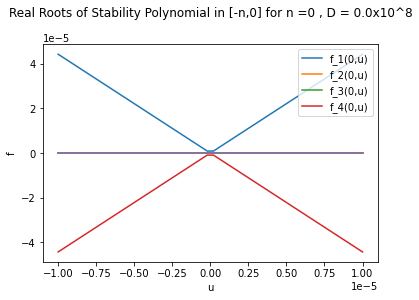
\includegraphics[width=.47\textwidth]{n0.png}\hfill
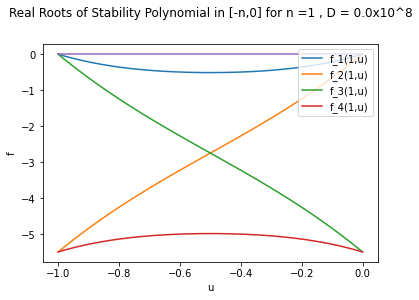
\includegraphics[width=.47\textwidth]{n1.png}\hfill
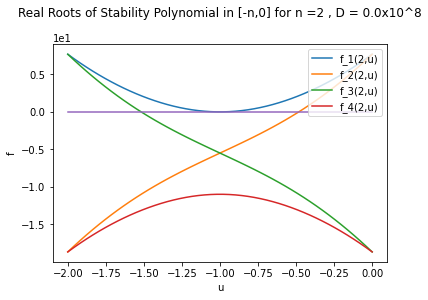
\includegraphics[width=.47\textwidth]{n2.png}\hfill
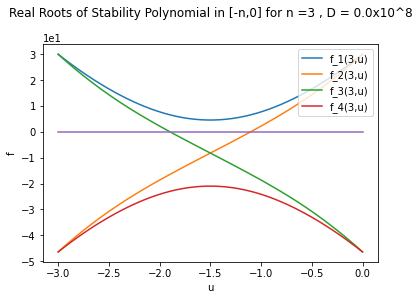
\includegraphics[width=.47\textwidth]{n3.png}\hfill
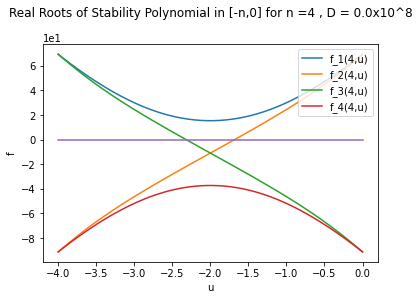
\includegraphics[width=.47\textwidth]{n4.png}\hfill
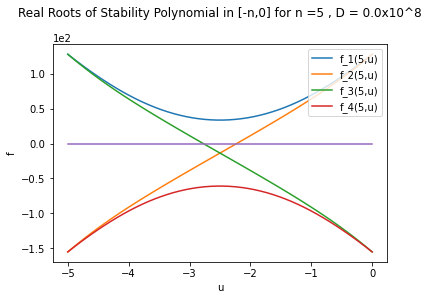
\includegraphics[width=.47\textwidth]{n5.png}\hfill
\caption{\emph{Spectral Stability Functions for n = 0 , 1, 2, 3, 4, and 5. The functions \(f_i\) correspond to the spectral stability functions \(p_i\) as defined in (\ref{p1}),(\ref{p2}),(\ref{p3}), and (\ref{p4}). Instability is possible when the spectral stability functions cross the purple line (y = 0) within the open Krein interval, and thus have real roots there. Here, blue corresponds to \(p_1\), yellow corresponds to \(p_2\), green corresponds to \(p_3\), and red corresponds to \(p_4\). Here, u is the Floquet parameter related to the period of the perturbation. It can be seen in these plots that as we increase n, roots are introduced into the open Krein interval (\ref{interval2}). Note that our Krein interval (\ref{interval2}) is an open interval, so the null interval in the n = 0 plot does not technically contain a root. The same can be said of the plot for n = 1, since the roots of \(p_1\), \(p_2\), and \((p_3)\) lie on the ends of the open interval. For all the plots where n \(>\) 1, we can see that \(p_2\) and \(p_3\) have valid roots in the interval.  Here, \(D = 0\) , \(\sigma = 0\), and \(h = 0.5\).}} \label{nvary}
\end{figure}



Generally, as D gets larger, the stability functions can develop new roots appearing in our interval (\ref{interval2}), The effects of variation of the surface flexural rigidity on the stability functions can be visualized in Figure \((\ref{Dvary})\). Note the qualitative similarity of the behaviour of the spectral stability functions to Figure (\ref{nvary}) as we now increase the D parameter, rather than the n parameter. \\

\begin{figure}[hbt!]
\centering
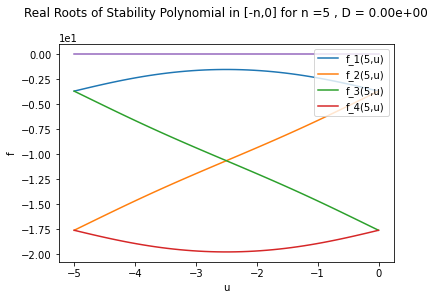
\includegraphics[width=.47\textwidth]{D0.png}\hfill
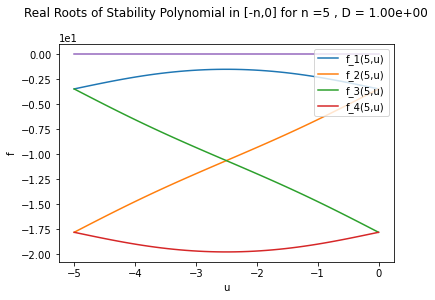
\includegraphics[width=.47\textwidth]{D1.png}\hfill
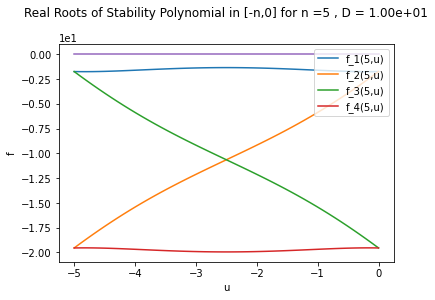
\includegraphics[width=.47\textwidth]{D2.png}\hfill
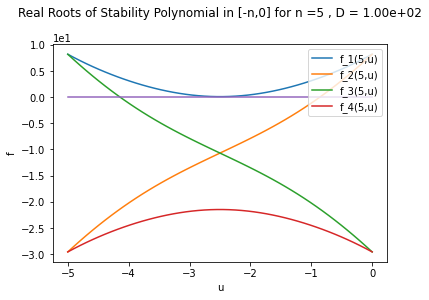
\includegraphics[width=.47\textwidth]{D2real.png}\hfill
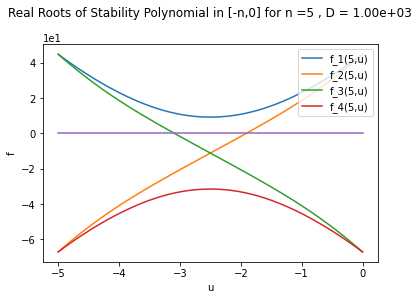
\includegraphics[width=.47\textwidth]{D3.png}\hfill
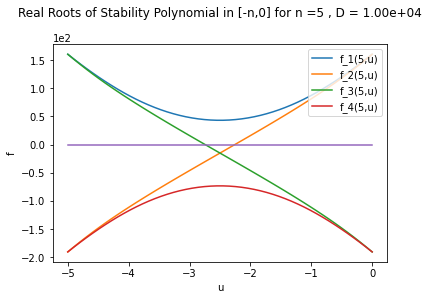
\includegraphics[width=.47\textwidth]{D4.png}\hfill
\vspace{-15}
\caption{\emph{Spectral Stability Functions for D = 0, 1, 10, 100, and 1000. The functions \(f_i\) correspond to the spectral stability functions \(p_i\) as defined in (\ref{p1}),(\ref{p2}),(\ref{p3}), and (\ref{p4}). Instability is possible when the spectral stability functions cross the purple line (y = 0) within the open Krein interval, and thus have real roots there. Here, blue corresponds to \(p_1\), yellow corresponds to \(p_2\), green corresponds to \(p_3\), and red corresponds to \(p_4\). Here, u is the Floquet parameter related to the period of the perturbation. It can be seen in these plots that as we increase D, roots are introduced into the open Krein interval (\ref{interval2}). Note that concerning applications to ice road safety, physical values of D lie in the range of MPa to GPa. The different values of D here are just to illustrate the relationship between D and real root existence in the Krein interval, namely that as D increases, real roots are introduced into the Krein interval. Here it is mainly \(p_2\) and \(p_3\) that have roots in the Krein interval, with the exception of n = 2 where there also exists a real root for \(p_1\). Here, \(n = 5\), \(\sigma = 0\), and \(h = 0.5\)}} \label{Dvary}
\end{figure}

\\



It can be seen that varying the surface tension \(\sigma\) throughout the physical regimes produces little to no discernible effect on the root behaviour of the spectral stability functions. This can be observed in Figure (\ref{sigmavary}) below. \\



\begin{figure}[hbt!]
\centering
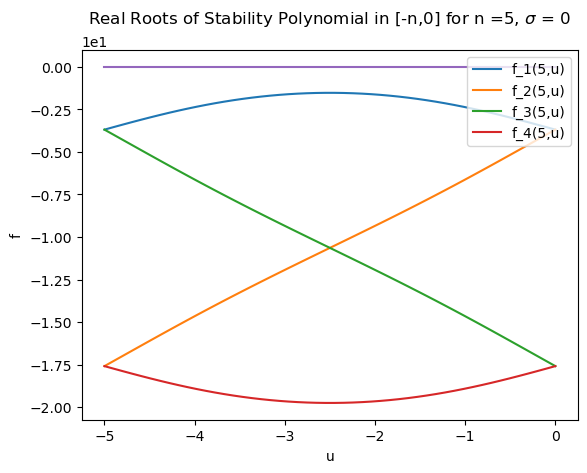
\includegraphics[width=.47\textwidth]{sigma1.png}\hfill
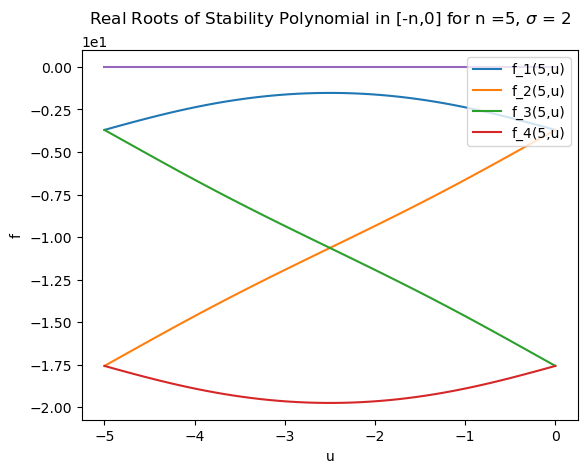
\includegraphics[width=.47\textwidth]{sigma2.png}\hfill
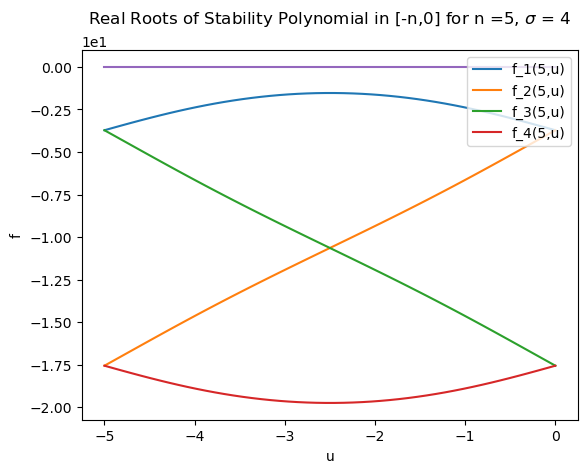
\includegraphics[width=.47\textwidth]{sigma3.png}\hfill
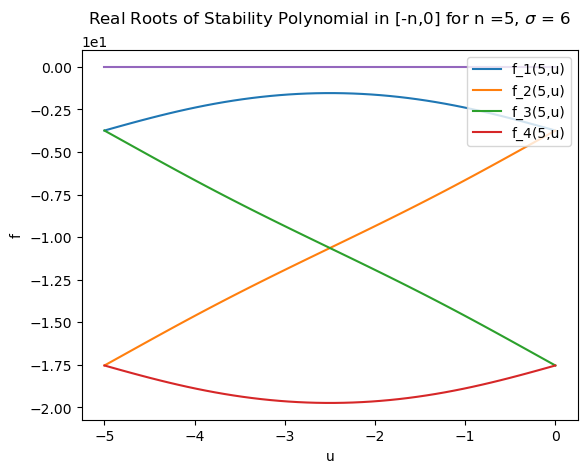
\includegraphics[width=.47\textwidth]{sigma4.png}\hfill
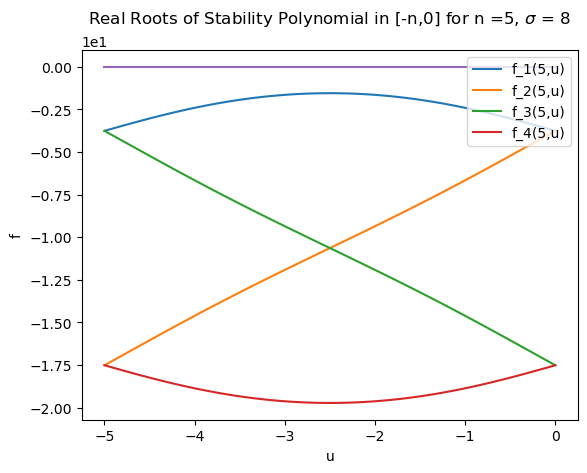
\includegraphics[width=.47\textwidth]{sigma5.png}\hfill
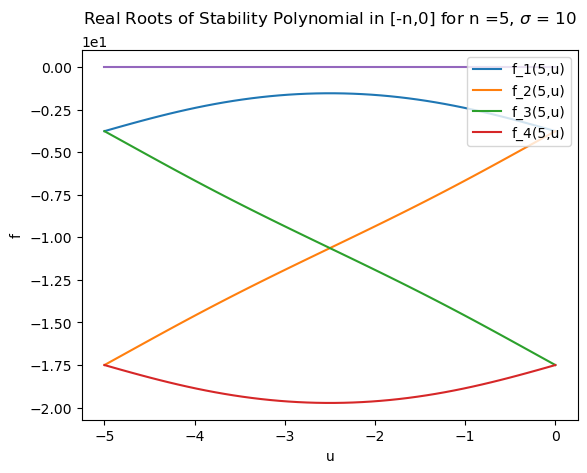
\includegraphics[width=.47\textwidth]{sigma6.png}\hfill
\vspace{-15}
\caption{\emph{Spectral Stability Functions for \(\sigma\) = 0, 2, 4, 6, 8, and 10. The functions \(f_i\) correspond to the spectral stability functions \(p_i\) as defined in (\ref{p1}),(\ref{p2}),(\ref{p3}), and (\ref{p4}). Instability is possible when the spectral stability functions cross the purple line (y = 0) within the open Krein interval, and thus have real roots there. Here, blue corresponds to \(p_1\), yellow corresponds to \(p_2\), green corresponds to \(p_3\), and red corresponds to \(p_4\). Here, u is the Floquet parameter related to the period of the perturbation. It can be seen in these plots that as we increase \(\sigma\), roots are not introduced into the open Krein interval (\ref{interval2}), and that the shape of the spectral stability functions are left essentially invariant. Here, \(n = 5\), \(D = 0\), and \(h = 0.5\)}} \label{sigmavary}
\end{figure}


\\
As the water depth parameter h goes to zero, the spectral stability functions approach the line \(y = 0\) as well, though this does not indicate instabilities because in this limit, the fluid domain ceases to exist when the water depth is non-existent. In the shallow water regime for our \(2\pi\) periodic waves, \(\frac{h}{\lambda} \leq 0.05\), the stability functions can exhibit root behaviour depending on the values of D, \(\sigma\), and n. Fixing these values, in the transitional \(0.05 \leq \frac{h}{\lambda} \leq 0.5\) and deep water regimes, \(\frac{h}{\lambda} \geq 0.5\), the spectral stability functions exhibit increased curvature that seems to introduce roots in the interval (\ref{interval}) in comparison with the shallow water regime. These results can be seen in Figure (\ref{hvary}). \\

\clearpage

\begin{figure}[hbt!]
\centering
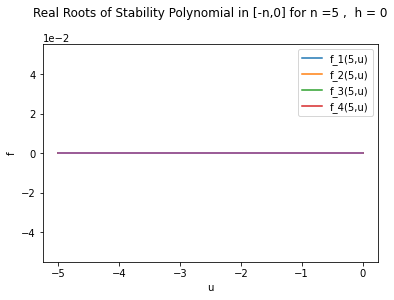
\includegraphics[width=.47\textwidth]{h1.png}\hfill
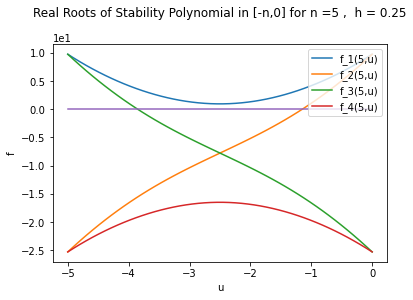
\includegraphics[width=.47\textwidth]{h2.png}\hfill
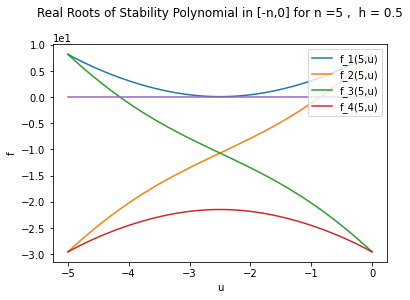
\includegraphics[width=.47\textwidth]{h3.png}\hfill
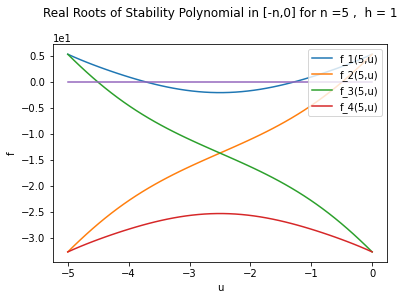
\includegraphics[width=.47\textwidth]{h4.png}\hfill
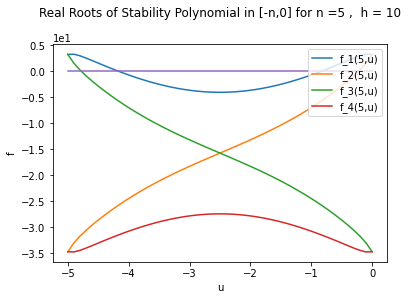
\includegraphics[width=.47\textwidth]{h5.png}\hfill
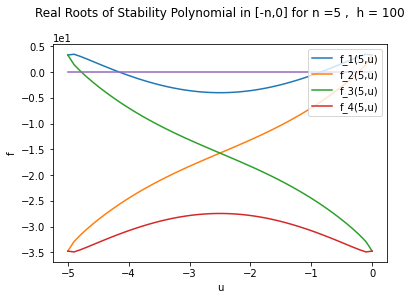
\includegraphics[width=.47\textwidth]{h6.png}\hfill
\vspace{-20}
\caption{\emph{Spectral Stability Functions for h = 0, 0.25, 0.5, 1, 10, and 100. Instability is possible when the spectral stability functions cross the purple line (y = 0) within the open Krein interval, and thus have real roots there. Here, blue corresponds to \(p_1\), yellow corresponds to \(p_2\), green corresponds to \(p_3\), and red corresponds to \(p_4\). Here, u is the Floquet parameter related to the period of the perturbation. The h = 0, and 0.25 graphs represent shallow water where \(\frac{h}{\lambda} \leq 0.05\). The h = 0.5, and 1 graphs represent transitional water where \(0.05 \leq \frac{h}{\lambda} \leq 0.5\). The h = 10, and 100 graphs represent deep water where \(\frac{h}{\lambda} \geq 0.5\). Remember that for our base solution, \(\lambda = 2 \pi\). Notice that for the h = 0 graph, our spectral stability functions are all equal to 0. It can also be seen that as we increase h, the \(p_1\) spectral stability function develops a root in the Krein interval, illustrating that real root existence can depend on water depth. Here \(n = 5\), \(D = 100\), and \(\sigma = 0\)}} \label{hvary}
\end{figure}



\\

\clearpage

\subsection{Varying Ice Thickness}

When performing the spectral stability analysis in Python, stability regimes were investigated upon varying the flexural rigidity D and Fourier mode difference parameter n. Since the range of D varies drastically on the order of \((1-10^9)\), instead of directly varying \(D\), we used our elasticity theory equation for surface-flexural rigidity (\ref{rigidity}) and varied the thickness of the ice denoted by d. The flexural rigidity is proportional to the thickness cubed as seen in (\ref{rigidity}), and thus evaluating stability regimes varying the thickness d with Fourier mode difference n offers a more instructive and clear comparison. \\

Stability outcomes were computed in Python for two different thickness regimes. In the millimeter regime, existence of real roots was checked numerically for approximately 2500 `coordinate' values of \((n,d)\), incrementally varying the parameters n and d at evenly spaced intervals. The same process was performed for the centimeter regime, but this time with \(10^4\) coordinate values, in order to encapsulate finer details of the stability boundaries in the regime. The figures below describe the stability outcomes for all coordinates for each regime, with red corresponding to unstable coordinates \((n,d)\) and blue corresponding to stable coordinates \((n,d)\). \\

\begin{figure}[hbt!]
\centering
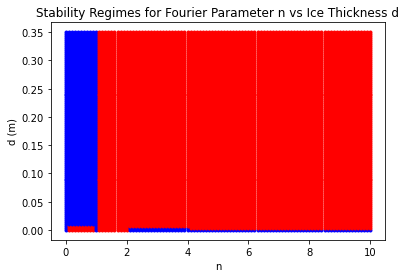
\includegraphics[scale = .8]{Stability CM .png}
\caption{ \emph{Stability regimes varying ice thickness in the centimeter regime with Fourier mode difference parameter n. Stable regions are denoted in "blue", whereas unstable regions are denoted in "red". Here, \(h = 0.5\), \(\sigma = 0\). }} \label{CM}
\end{figure}


\begin{figure}[hbt!]
\centering
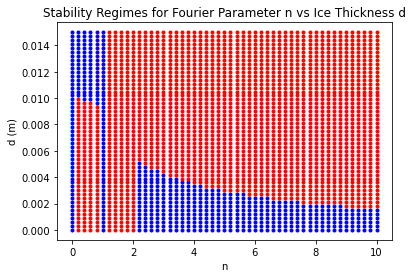
\includegraphics[scale = .8]{Stability MM.png}
\caption{\emph{Stability regimes varying ice thickness in the millimeter regime with Fourier mode difference parameter n. Stable regions are denoted in "blue", whereas unstable regions are denoted in "red". Here, \(h = 0.5\), \(\sigma = 0\)}} \label{MM}
\end{figure}

\\

\clearpage

\subsection{Different Resonant Modes}

Upon investigating resonance regimes, the resonance condition (\ref{resonance}) was found to be satisfied for all D for values of \(K = 1\) and \(K = 0\), though the first case is forbidden by (\ref{resonance}). \(K = 0\) is also a rather trivial case since physically, it simply represents flat water. There also exists a value of K satisfying (\ref{resonance}) that varies as the ice thickness d (or surface flexural rigidity D) is varied. Let us call this mode K'. The dependence of K' on the ice thickness d is demonstrated below in Figure (\ref{Kmode}).  \\

\begin{figure}[hbt!]
\centering
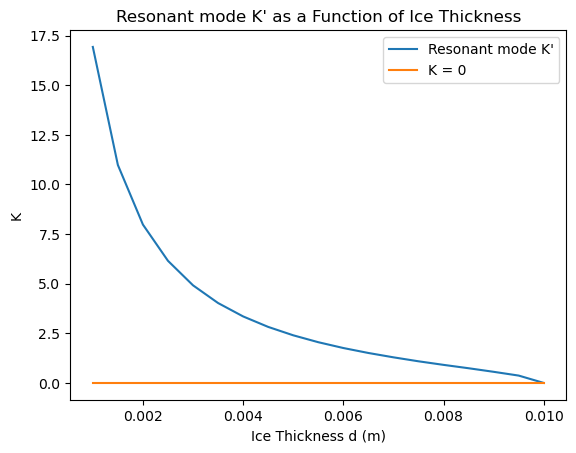
\includegraphics[scale = .8]{Resonant.png}
\caption{\emph{Resonant mode K' as a function of ice thickness d. By (\ref{rigidity}), K' is dependent on flexural-rigidity as well. Note that as d approaches 1 centimeter, the resonant mode K' collides with the aforementioned D-independent mode at \(K = 0\). Here, \(h = 0.5\), \(\sigma = 0\)}} \label{Kmode}
\end{figure}
\\

We can also visualize this relationship by investigating the real roots of the spectral stability function for various values of d in the millimeter regime, and seeing how close the roots are to matching the resonant mode K'. Resonance will not generally occur for non-integer modes, but near-resonances, that is, near-collisions of the mode K' and the real roots of the spectral stability functions can occur for non-integer modes. These near-resonances are depicted below in Figure (\ref{nearres}).
\\

\begin{figure}[hbt!]
\centering
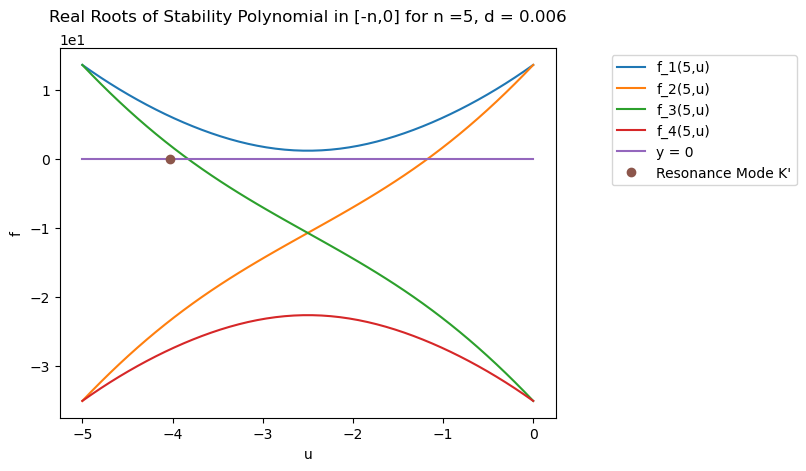
\includegraphics[width=.8\textwidth]{k2.png}
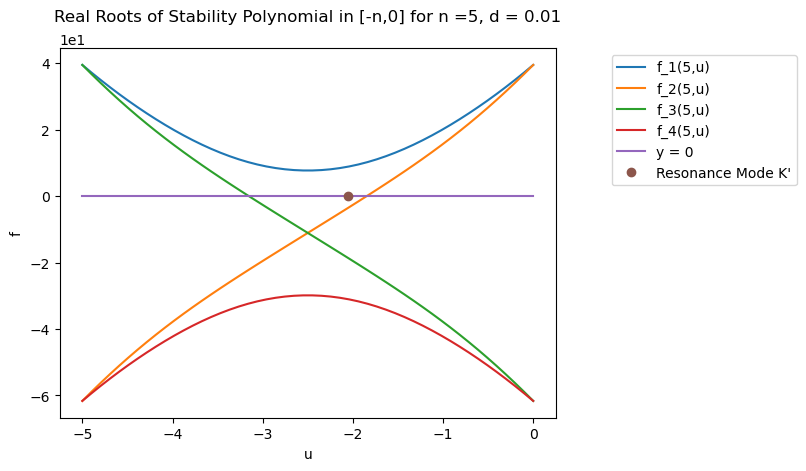
\includegraphics[width=.8\textwidth]{k6.png}\hfill
\caption{\emph{Spectral Stability Functions for \(d = 6\) mm and \(d = 10\) mm, plotted alongside resonant mode K' for each value of d. Notice the near-collisions of the K' mode with the real roots of the spectral stability functions. Here \(n = 5\), \(h = 0.5\), and \(\sigma = 0\)}} \label{nearres}
\end{figure}
\\

\clearpage


We now focus our attention on the stability of our system under some special cases of the parameters D, \(\sigma\), h, and n. We chose to examine the special cases of \(n=2\) and \(n=1\) due to the observed stability regimes in Figures (\ref{CM}) and (\ref{MM}). 

\subsection{The Unstable Regime of n = 2}
\\

For all values of D, \(\sigma\), and h, it can be observed that there exists a real root in the interval (\ref{interval2}) for \(n = 2\), and thus the system can have instabilities here for all values of D, \(\sigma\), and h. This real root occurs at \(\mu = -1\), which also happens to satisfy the resonance condition (\ref{resonance}) for all values of D, \(\sigma\), and h. Examples of the instabilities at n = 2 are demonstrated in Figure (\ref{n=2}). It is also of note that in Figure (\ref{CM}), it can be seen that for values of n such that \(1 \leq n \leq 2\), we have the same unstable behaviour of the system. However, we focus on the \(n=2\) case here because it represents a boundary for this unstable regime, as can be seen in Figure (\ref{CM}). 
\\

\begin{figure}[hbt!]
\centering
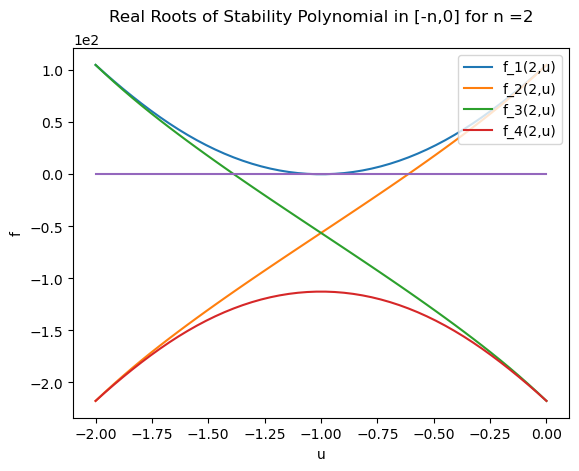
\includegraphics[width=.5\textwidth]{special1.png}\hfill
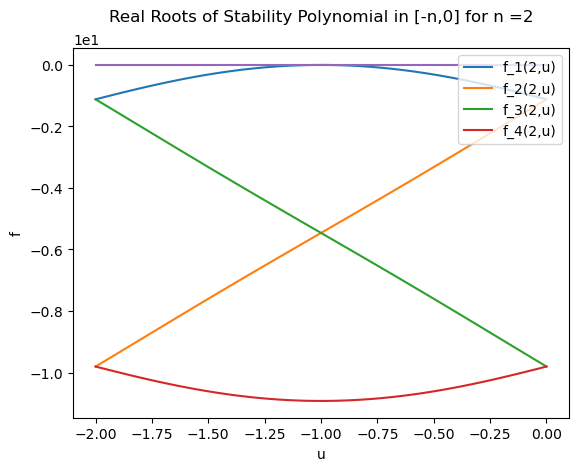
\includegraphics[width=.5\textwidth]{special2.png}\hfill
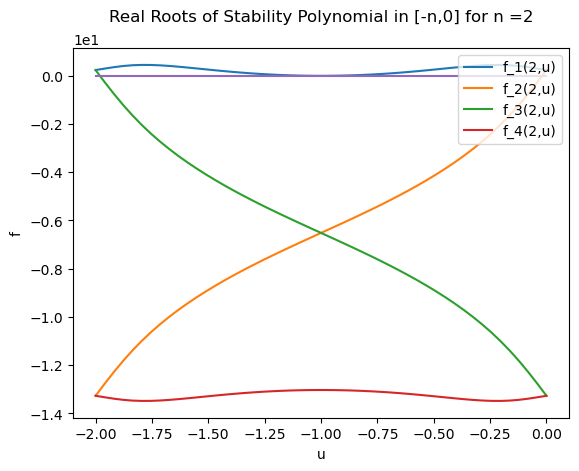
\includegraphics[width=.5\textwidth]{special3.png}\hfill
\caption{\emph{Spectral Stability Functions for n = 2. The top left graph has parameters h = 10, \(\sigma = 0\), d = 0.01, \(D = 8.1 \times 10^5\). The top right graph has parameters h = 1, \(\sigma = 7\), d = 0.001, \(D = 0.81\). The bottom graph has parameters h = 5, \(\sigma = 0\), d = 0.01, \(D = 813\). Note that for all graphs, there exists a root at \(\mu = -1\), and thus all of these parameter configurations can have instabilities. }} \label{n=2}
\end{figure}
\\

\subsection{The Stable Regime of n = 1}

Now, consider \(n = 1\). For all values of D, \(\sigma\), and h, it can be observed that there exists solely two real roots on the boundaries of the interval (\ref{interval2}) for \(n = 1\). The interval is open though, and thus these roots do not constitute possible instabilities of the system since the Krein condition is not satisfied. Thus, for \(n = 1\), all combinations of parameters D, \(\sigma\), and h yield stable solutions. The real roots occur at \(\mu = -1\) and \(\mu = 0 \), which also happen to satisfy the resonance condition (\ref{resonance}) for all values of D, \(\sigma\), and h. Examples of the stabilities at n = 1 are demonstrated in Figure (\ref{n=1}). 
\\

\begin{figure}[hbt!]
\centering
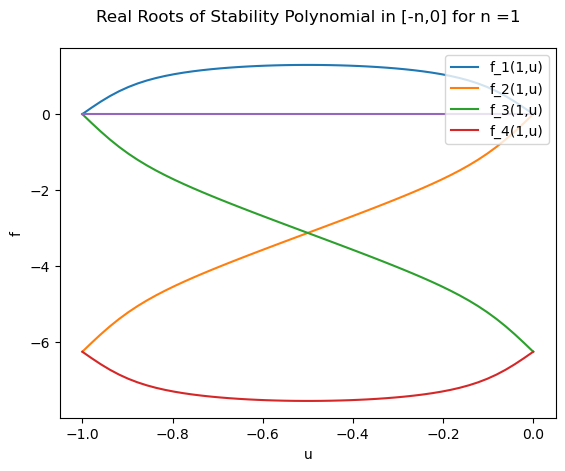
\includegraphics[width=.5\textwidth]{special4.png}\hfill
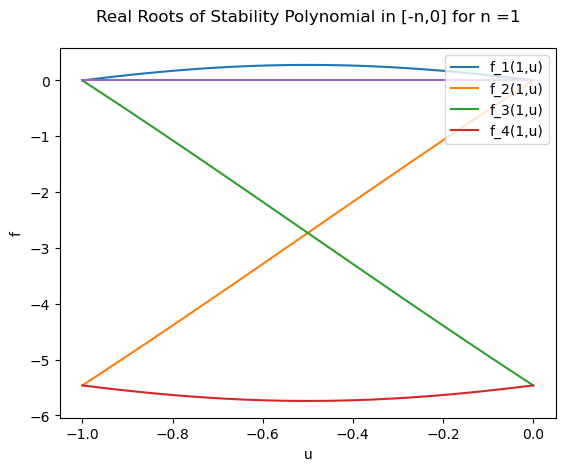
\includegraphics[width=.5\textwidth]{special5.png}\hfill
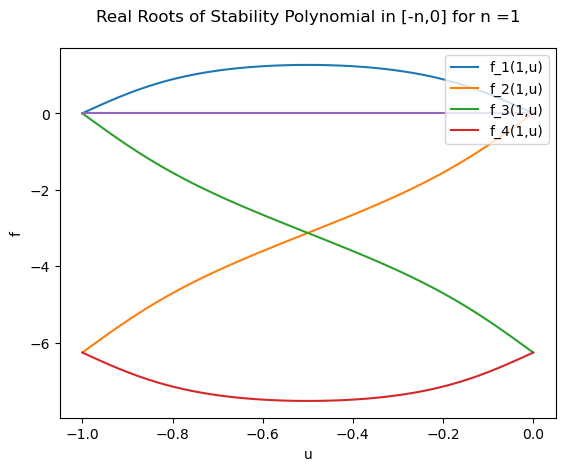
\includegraphics[width=.5\textwidth]{special6.png}\hfill
\caption{\emph{Spectral Stability Functions for n = 1. The top left graph has parameters h = 10, \(\sigma = 0\), d = 0.1, \(D = 8.1 \times 10^5\). The top right has parameters h = 1, \(\sigma = 7\), d = 0.001, \(D = 0.81\). The bottom graph has parameters h = 5, \(\sigma = 0\), d = 0.01, \(D = 813\). Note that for all graphs, there exists roots at \(\mu = -1,0\) which are not inside the open Krein interval, and thus all of these parameter configurations are stable. }} \label{n=1}
\end{figure}
\\

\clearpage 

\section{Discussion}
By considering Figures (\ref{CM}) and (\ref{MM}), we determined that we have stability in our system for \(n = 1\), and that for all other values of n, our system can exhibit instabilities. It should be noted that for \(n \leq 1\), the system is stable for all values of d in the centimeter ice thickness range. In the millimeter range, there are more complicated regimes of instability and stability depending on various combinations of d and n. We discuss how these stability regimes depend on the physical parameters of the system below.

\subsection{Varying D, \(\sigma\), and h}

When D is large, it has drastic effects on the spectral stability functions since the surface flexural term is multiplied by the highest order term \(\mu ^ 5\), and thus dominates the expression as D becomes even remotely large. Furthermore, since the physical range of D is so large (on the order of \(10^9  N \cdot m^2\)), it makes sense that the surface flexural term dominates in the stability analysis for most physical values of D. It is consistent with the literature that for higher values of the surface flexural rigidity, we obtain more high frequency instabilities in the water-wave ice system. For example, the increase of instabilities with increasing values of surface-flexural rigidity D is a finding that is similar to the results of the 2D flexural-gravity deep water stability analysis previously done by Trichtchenko [\ref{olga1}]. A physical mechanism for this proportionality is currently up for speculation, though it should be noted that a lot of wave solutions under ice are unstable and thus will not be frequently seen in nature [\ref{olga1},\ref{bandstructure}]. However, when these unstable waves do exist, they can break the ice. 
\\
\\


When \(\sigma\) is varied, it can be observed that since physical regimes for this parameter vary from approximately 0 to 7 \(N \cdot m\), it follows that since \(\sigma\) is divided by \(\rho = 1000 \frac{kg}{m^3}\) in the spectral stability functions, the magnitudes for terms containing sigma are always small compared to that of the D and g terms, and thus it makes sense that varying \(\sigma\) produces no effects on the stability. Physically, if we have a non-zero \(\sigma\), this implies the non-existence of ice on the water surface, and thus the problem we are studying reduces to the case of capillary-gravity water waves simply moving along the interface between water and air. It is of note that the high frequency instabilities that we are studying do not occur in this regime. Our finding reflects the fact that lots of capillary-gravity waves are stable, and many different kinds can be seen in nature [\ref{cap1} - \ref{cap4}]. 
\\
\\

When h is varied to be in the deep water regime (\(\frac{h}{\lambda} \geq 0.5\)), it was noted that varying h introduced extra roots in the spectral stability functions. The root behaviour of the spectral stability function should not depend strongly on h, since h only really comes into the spectral stability functions as a scaling term in the hyperbolic tangent function, and not as a parameter that shifts the intercepts of the function. However, it can be seen that for certain parameters like the parameter configuration in Figure (\ref{hvary}), such scaling of h can introduce roots into the system. Since the stability of the particular solutions to the water wave problem have been studied already in the deep and shallow water regime, the majority of our results were computed in the transitional water regime \(0.05 \leq \frac{h}{\lambda} \leq 0.5\). 
\\
\\

\subsection{Millimeter Regime}

Looking at our comparison of d and n values in the centimeter regime for ice thickness d, Figure (\ref{CM}) essentially zooms in on the interesting stability regimes in the bottom left quadrant of Figure (\ref{MM}). It is of note that we can see the effect we had previously discussed of total stability here at \(n = 1\) for all values of d. 
\\

Here, we can see a regime of stability for n greater than 2 and d less than 6 millimeters. This regime of stability most likely accounts for the fact that when d is this small, the surface flexural rigidity term is comparable in magnitude to the gravity term, and thus does not dominate yet in the spectral stability functions. We previously mentioned that these high-frequency instabilities increase with increasing values of D. As the ice thickness d increases, the surface-flexural rigidity D term increases to the power of three, and thus starts to dominate in it's contribution to the spectral stability functions, yielding real roots in the Krein interval (\ref{interval2}), and thus instability of the system. In Figure (\ref{CM}), we can see a sort of sloping cut-off curve for the stability where for a given value of n greater than 2, if d is sufficiently large, the high frequency instabilities begin to become possible, with higher values of n instabilities occurring at lower cut-off thresholds for the ice thickness. The implication of this is that these high-frequency instabilities tend to favour larger differences in frequency over smaller differences in frequency when comparing the dominant plane wave modes in the Fourier-Floquet expansion (\ref{floquet}) comprising our perturbation. A mathematical explanation for this is that raising the Fourier parameter n causes the spectral stability functions (\ref{p2}) and (\ref{p3}) to exhibit root behaviour that converges closer and closer to the midpoint of the interval (\ref{interval2}) for increasing n. A physical interpretation is purely speculative, but may be due to a sort of constructive interference between the plane wave components of the perturbation that grows with increasing values of n.
\\
\\


\subsection{Centimeter Regime}
\\

Note that in the methodology, we showed that the existence of real roots in the Krein interval (\ref{interval2}) is equivalent to satisfaction of the Krein condition. Satisfaction of the Krein condition (\ref{krein2}) is a necessary condition for high-frequency instabilities of the water wave problem, and our findings here in Figure (\ref{CM}) support that notion. Looking at our comparison of d and n values in the centimeter regime for ice thickness d, it can be seen that for most values of d and n in Figure (\ref{CM}), our system can have instabilities. This is because as the ice thickness increases slightly, the surface flexural rigidity term increases dramatically to the power of three and has the effect of drastically compressing the spectral stability functions such that for most values of d and n, there exists roots in the interval (\ref{interval2}), and thus the Krein condition is satisfied, and so we can have instability. 
\\

Looking to Figure (\ref{CM}), we can discuss the following result. For sufficiently large d, there exists a bifurcation at the vertical line \(n = 1\) that separates the (n,d) plane into stable and unstable regions. For n less than 1, it is of note that this entails guaranteed stability for ice thickness d greater than 1 cm for our fixed values of \(h = 0.5\) and \(\sigma = 0\). It is interesting to observe that our system is stable for Fourier mode differences \(n<1\). These stabilities occur in this regime because for these values of n, the spectral stability functions (\ref{p1}), (\ref{p2}),(\ref{p3}), and (\ref{p4}) do not exhibit real roots in the interval (\ref{interval2}), and thus this implies that the Krein instability condition (\ref{krein2}) is not satisfied. Since this condition is not satisfied, it is impossible for our system to exhibit instabilities for \(n<1\), and so the system is stable. Examining the other regime of this bifurcation where \(n > 1\), we notice that real roots of the spectral stability functions do exist however for \(n>1\), and thus instabilities are possible in this n regime. Looking at Figure (\ref{CM}), the upper right unstable regime implies that for d greater than 1 cm, instabilities can essentially only be generated by waves travelling with differences in Fourier mode greater than the value of our initial \(k = 1\) mode. \\



A possible physical explanation for both regions of the bifurcation echoes the sentiments of the section above, where a form of constructive interference correlated with increasing n may be occurring to explain the instabilities for \(n>1\). Furthermore, with decreasing n, one might theorize that the amplitudes of the flexural-gravity waves experience a decrease in this `spectral' constructive interference, so much so that there exists a threshold \((n = 1)\) such that the system experiences the bifurcation, and the amplitudes for \(n < 1\) tend to zero rather than infinity. 
\\

Since the centimeter ice thickness regime is the most physically relevant regime for our ice-water wave problem, we will now discuss the implications of this bifurcation at \(n = 1\). This bifurcation reflects the fact that these instabilities are truly high frequency instabilities, which we illustrate with a 3D plot of the the function \(n = |l - m| = |\frac{2 \pi}{\lambda} - \frac{2 \pi}{\zeta}|\) in Figure (\ref{specialn}) below, where \(\lambda\) and \(\zeta\) correspond to the wavelengths of the l and m modes, respectively. By plotting this function on top of the plane \(n = 1\) corresponding to the bifurcation, we can split the 3D space \((\lambda,\zeta,n)\) into an upper region \(n>1\) of instability, and a lower region \(n<1\) of stability. It can be noted that since the Fourier modes are inversely proportional to the wavelengths of the plane waves in the perturbation \((k = \frac{2\pi}{\lambda})\), that means they are proportional to the frequencies of the plane waves by \(f = \frac{c}{\lambda}\). Note c here is not constant because these are dispersive waves, but we can ignore the effects of dispersion here because our wave speed (\ref{cp}) is also inversely proportional to wavelength, which gives us an approximate relation \(f \sim \frac{1}{\lambda^2}\) and is thus still an inverse proportionality for frequency to wavelength. \\

In Figure (\ref{specialn}) below, we can see that for a low wavelength regime corresponding to small values of the coordinates \((\lambda,\zeta) \in \{\lambda^2 + \zeta^2 \leq 5| \hspace{2} \zeta \geq 0, \lambda \geq 0\}\), small differences in wavelengths can generate instabilities, and thus the unstable regime is more prevalent, since the majority of the green-coloured function \(n = |l - m|\) is above the bifurcation plane at \(n = 1\). For a large wavelength regime corresponding to large values of the coordinates \((\lambda,\zeta) \in \{\lambda^2 + \zeta^2 \geq 5|  \hspace{2}  \zeta \geq 0, \lambda \geq 0\}\), it takes large differences in wavelengths in order to generate these instabilities, and thus the stable regime is more prevalent since the majority of the green-coloured function \(n = |l - m|\) is beneath the bifurcation plane at \(n = 1\). Since the low wavelength regime is equivalent to the high frequency regime, and the low wavelength regime is the regime of prevalent instabilities, these are truly high-frequency instabilities we are observing, thus echoing the pre-existing results from the literature [\ref{olga1},\ref{katie},\ref{bernardd}]. \\

Since \(h = 0.5\) metres here, the deep water regime \((\frac{h}{\lambda} \geq 0.5)\) is for wavelengths less than 1 metre here. The transitional water regime \((0.05 \leq \frac{h}{\lambda} \leq 0.5)\) is for wavelengths between 1 and 10 metres, and the shallow water regime \((\frac{h}{\lambda} \leq 0.05)\) is for wavelengths greater than 10 metres. Thus, these high-frequency instabilities would most commonly occur in the deep water regime, and slowly become less common as the wavelength increases through the transitional regime to the shallow water regime. However, in the model that we are considering, we are simply in transitional water with our base mode \(\lambda = 2 \pi\) and \(h = 0.5\), and the plane wave components in the perturbation model a moving load on the ice, rather than naturally occurring waves in the water. 

\begin{figure}
    \centering
    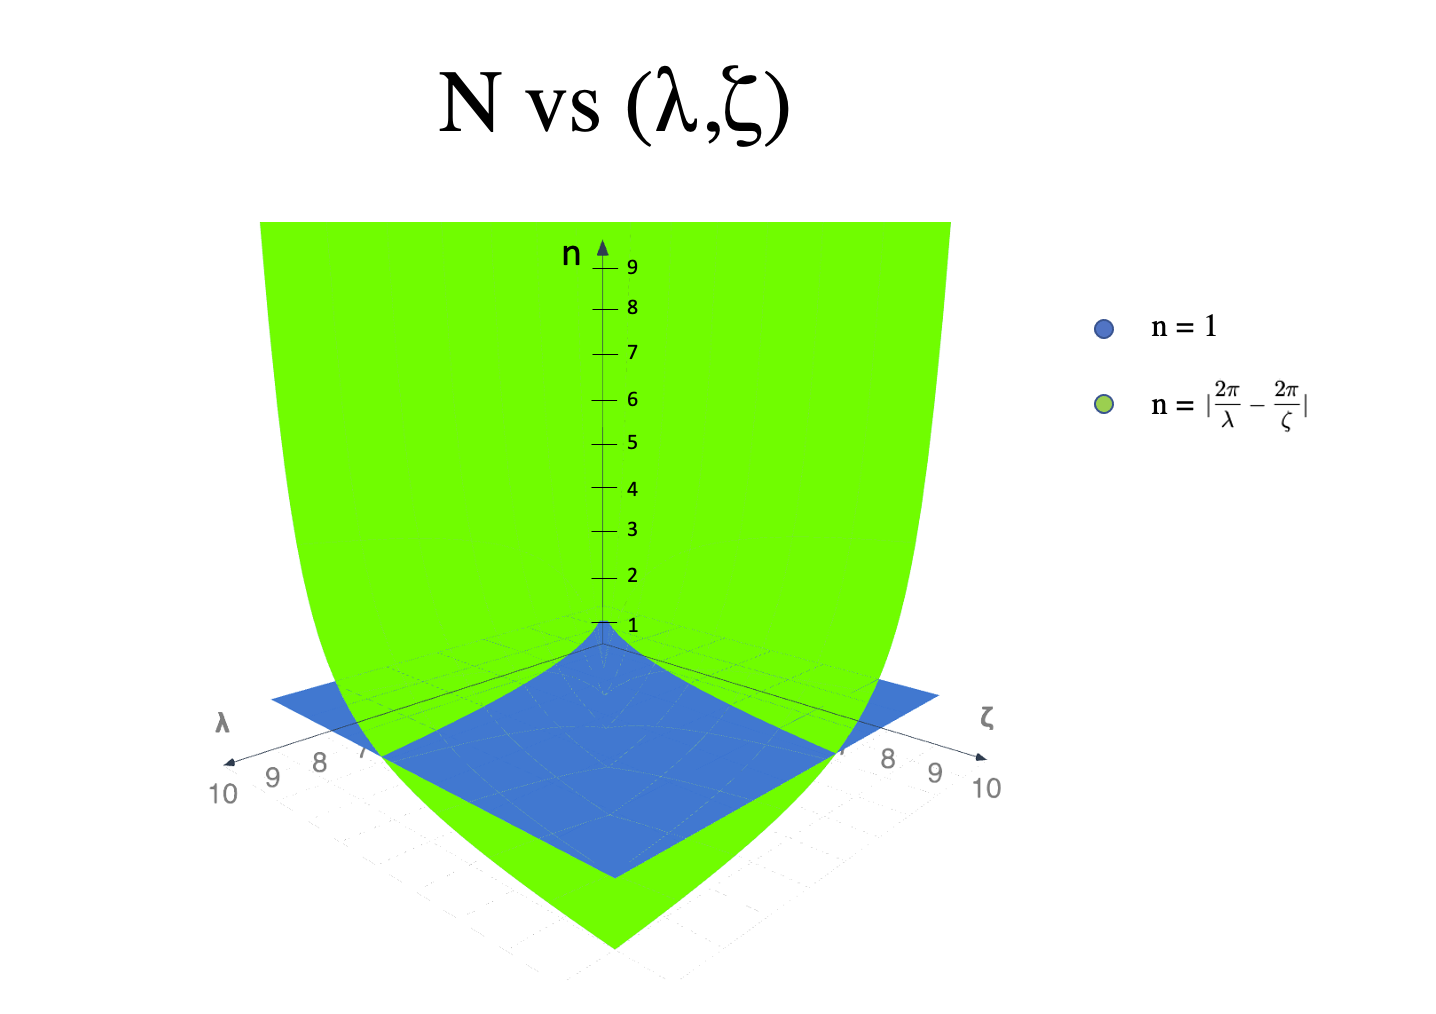
\includegraphics[width=.7\textwidth]{specialn.png}\vfill
    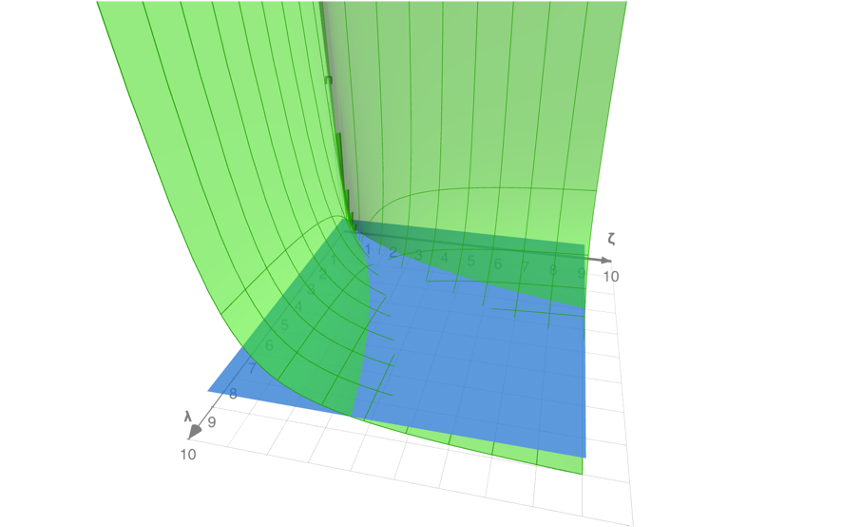
\includegraphics[width=.45\textwidth]{version2.png}
    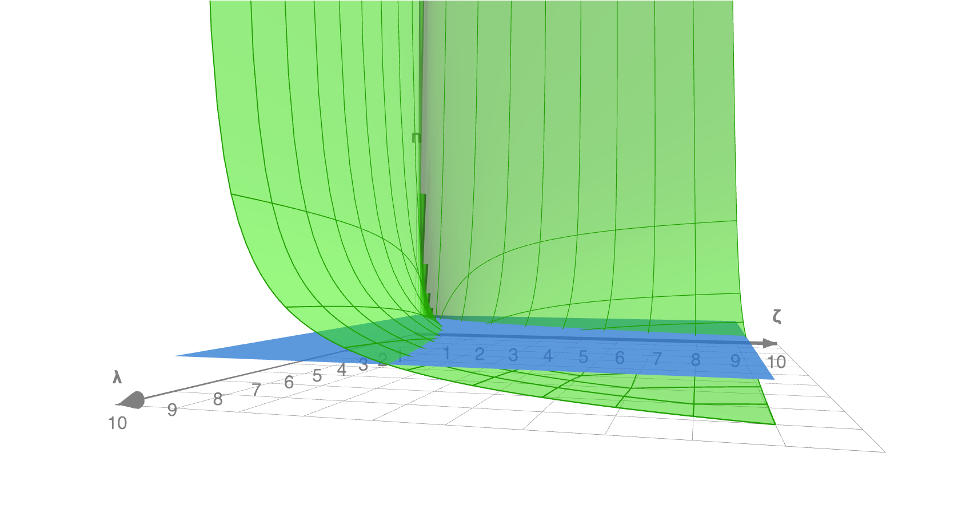
\includegraphics[width=.5\textwidth]{version3.png}\hfill
    \caption{\emph{Fourier mode difference parameter \(n = |l - m| = |\frac{2 \pi}{\lambda} - \frac{2 \pi}{\zeta}|\) versus wavelengths of two different perturbation modes in the centimeter ice thickness regime (transitional water). Here, the \(\lambda\) axis corresponds to the wavelength of the l mode \((l = \frac{2\pi}{\lambda})\), and the \(\zeta\) axis corresponds to the wavelength of the m mode \((m = \frac{2\pi}{\zeta})\). Note that \(n = |l-m|\) has been plotted in green, and the stability bifurcation plane \(n = 1\) has been plotted in blue. Coordinates of the green surface above the blue plane correspond to unstable regimes with \(n>1\), whereas coordinates of the green surface below the blue plane correspond to stable regimes with \(n<1\). The takeaway from this plot is that for large values of the perturbation mode wavelengths \(\lambda\) and \(\zeta\) (points on the plot far from the origin), stability is more prevalent, since the majority of the green plot is beneath the blue plane \(n=1\). For smaller values of \(\lambda\) and \(\zeta\) (points close to the origin), instability is more prevalent, since the majority of the green plot is above the blue plane. The bottom two graphs just give different 3D perspectives to illustrate the dominance of the green surface \(n = |l-m|\) for small wavelengths (instabilities are more common), and the dominance of the blue surface \(n = 1\) for large wavelengths (stabilities are more common).}}
    \label{specialn}
\end{figure}


\subsection{Resonant Mode}
\\
\\
Examining our results for the K' resonant mode, it is of note that as the thickness d increases to 1 cm, the resonant mode K' collides with the D-independent mode at \(K = 0\). Note that this is the exact cut off point for the little rectangular regime of instability in the bottom left corner of Figure (\ref{CM}) for the same parameter values of \(h = 0.5\) and \(\sigma = 0\). It is possible that this unstable regime is partially due to the presence of this K' resonant mode for values of d less than 1 cm. It can be noted that for the fixed parameters \( n = 5\), \(\sigma = 0\), and \(h = 0.5\), as one varies d from 1 mm to 6 mm, one can observe near-resonant collisions in the interval (\ref{interval2}) which may cause sort of pseudo-resonant amplitude spiking of the flexural gravity waves, and thus instability in this regime. 

\\
\\

\subsection{Total Stability for \(n = 0,1\)}
For the case where \(n = 1\) and for all values of D, \(\sigma\), and h, we observed that there will always exist roots only at the endpoints of the interval (\ref{interval2}). Since there does not exist real roots actually \emph{inside} this interval, it follows that for all configurations of the parameters where \(n = 1\), our system is stable here. It is curious that perturbations with differences in Fourier mode of one do not create instabilities in this system. Physically, this implies that we always get stability when perturbing our high-frequency zero'th order solution with a perturbation solely composed of two plane waves components with Fourier modes differing by one. This unity is rather artificial and arises from our convenient choice of \(2\pi\) wavelength of our initial mode \(k = \frac{2\pi}{\lambda} = 1\), but it is interesting nonetheless, since we have all values of n in a neighborhood around \(n = 1\) yielding unstable regions for the millimeter regime as seen in Figure (\ref{MM}), as opposed to the stability regime of the vertical line at \(n = 1\). 
\\

For the case where \(n = 0\) and for all values of D, \(\sigma\), and h, we find that we will always trivially have stability (\ref{interval2}). Since the open interval collapses to a point at the origin, it follows that for all configurations of the parameters where \(n = 0\), there can not exist roots in the interval since the interval no longer exists, and so the Krein condition can never be satisfied, and thus our system is stable here. This is as expected since our perturbation will have the greatest contribution from the mode \(k = 1\) which we chose from the outset, and so we expect that perturbation plane waves with mode equal to \(k = 1\) (and thus \(n=k-k=0\)) would always be stable since our system starts off as stable. 
\\
\\


\subsection{Total Instability for \(n = 2\) and Resonant Effects}
For the case where \(n = 2\) and for all values of D, \(\sigma\), and h, we observed that there will always exist roots at the midpoint of the interval (\ref{interval2}), and that this root happens to also satisfy the resonance condition. Therefore, not only can this system undergo the instabilities we've been studying so far, but it can also cause our system to experience resonance, which can cause amplitudes to grow dramatically and potentially break the ice. To give a physical example, suppose our perturbation has a Floquet parameter \(\mu\) of 0, and that our perturbation is of the simplest form such that it satisfies n = 2, that is, a single plane wave with m = -1, so \( N = \mu + m = 0 - 1 = -1\). Thus noting that our zero solution has \( k = 1\), we have \(n = |k - N| = 2\) as required, and our perturbation term \(q^{(1)}\) can be written using (\ref{q2}) as:

\begin{equation} \label{q3}
  q^{(1)}(x,t) = (b_{-1})\delta_{0}e^{\lambda t}e^{-i(x-V_{0}t)}
\\
\end{equation} 

so that using our expression for the linear perturbation velocity (\ref{cp}) with \(N = -1\), we recover:

\begin{equation} \label{cp}
  c_{p} = \pm \frac{\sqrt{(g(-1) - \frac{\sigma(-1)^3}{\rho} + \frac{D(-1)^5}{\rho})\tanh{(-h)}}}{-1} 
\\
\end{equation} 

which implies (taking the negative sign corresponding to propagation of the load in the negative \(\hat{x}\) direction):

\begin{equation} \label{cp2}
  c_{p} = \sqrt{(g - \frac{\sigma }{\rho} + \frac{D }{\rho})\tanh{(h)}} = V_{0}
\\
\end{equation} 

but this is the exact expression we found for the wave speed (\ref{V}), so that means that \(|c_{p}| = |V_0|\) and thus the resonance condition (\ref{resonance2}) is satisfied. Therefore, our perturbation for q is specified here such that the flexural-gravity waves undergo high-frequency instabilities that may also break the ice at critical amplitudes via the resonance method of ice destruction.
\\
\\


\section{Conclusion}

In summation, upon variation of the parameters D, \(\sigma\), and h individually, while holding the others constant, we found that there exists changes in stability only under variation of the surface flexural rigidity D for flexural-gravity waves, and not the surface tension \(\sigma\) for capillary-gravity waves. We found that as D increases, so do the number of eigenvalue collisions representing real roots in the Krein interval, and thus instabilities of the system. The ice thickness d and the Fourier mode difference parameter n were varied simultaneously in the millimeter and centimeter regimes of d. In the centimeter regime, a bifurcation between the unstable regime and the stable regime along the line \(n = 1\) was found such that for sufficiently large d, there exists a regime of stability for all \(n<1\) and a regime of instability for all \(n>1\). We found that these instabilities were truly in the  high-frequency range, echoing the results of pre-existing studies for flexural-gravity waves. In the millimeter range for d, we found a regime of stability for \(n>2\) and sufficiently low ice thickness, with the instability cutoff thickness decreasing with increasing n. We found a regime of instability for \(0 < n < 1\), and sufficiently low ice thickness d. We also found a resonant mode K' that decreases with increasing ice thickness d and exhibits near-resonant high-frequency instabilities if K' is in the open Krein interval prescribed by the Krein signature condition. We also found stable regimes under variation of all parameters for \(n = 0\), \(n = 1\), as well as an unstable regime under variation of all parameters for \(n = 2\), with a real root in the Krein interval that always satisfies the resonance conditions (\ref{resonance}) and (\ref{resonance2}), and thus is an example in our system of the phenomena of the resonance method of ice destruction. In conclusion, upon implementation of this perturbative stability analysis generalizing the methods of Trichtchenko et. al [\ref{olga1}], we have classified spectral stability regimes of the water wave problem, with a focus on the transitional water regime and ice thickness values in the millimeter and centimeter ranges.
\\

\section{Acknowledgements}
\\ 
Many thanks to Dr. Katie Oliveras, Associate Professor of Mathematics at Seattle University for her guidance with technical details of the AFM formulation of the water-wave problem. Thanks to Bernard Deconninck, J.-M. Vanden-Broeck, P. Milewski and E. Parau for their illuminating findings in their respective resesarch in the stability of water waves. Lastly, I'd like to express my gratitude to Dr. Olga Trichtchenko and Dr. Giovanni Fanchini for their continued support and guidance throughout the term -- this was one of my favourite experiences in my undergraduate degree.

\clearpage

\subsection{References}
\\
\begin{enumerate}
\small{
\item{Trichtchenko, Olga, et al. “Stability of Periodic Travelling Flexural-Gravity Waves in Two Dimensions.” ArXiv.org, 29 Jan. 2018, arxiv.org/abs/1801.09748.} \label{olga1} \\

\item{Trichtchenko, Olga. “A Method for Identifying Stability Regimes Using Roots of a Reduced-Order Polynomial.” SpringerLink, Birkhäuser, Cham, 1 Jan. 1970, \(link.springer.com/chapter/10.1007/978-3-030-33536-6_12\).} \label{reduced}\\

\item{Nonlinear Dynamics and Chaos: with Applications to Physics, Biology, Chemistry, and Engineering, by Steven H. Strogatz, CRC Press, 2019.} \label{stabilitypde} \\


\item{Yirka, Bob. “Study Suggests Large Waves May Have Bigger Role in Breaking up Polar Sea Ice than Thought.” Phys.org, Phys.org, 29 May 2014, phys.org/news/2014-05-large-bigger-role-polar-sea.html.} \label{icewavespic} \\

\item{Trichtchenko, Olga, et al. “The Instability of Wilton Ripples.” Wave Motion, Elsevier, 22 June 2016, \\ www.sciencedirect.com/science/article/pii/S0165212516300592. \label{wilton}} \\

\item{Chou, Tom. “Band Structure of Surface Flexural–Gravity Waves along Periodic Interfaces: Journal of Fluid Mechanics.” Cambridge Core, Cambridge University Press, 25 Aug. 1998, www.cambridge.org/core/journals/journal-of-fluid-mechanics/article/band-structure-of-surface-flexuralgravity-waves-along-periodic-interfaces/8C78D8086BB5013F0340D\\5C970B416E7.} \label{bandstructure} \\


\item{Deconinck, Bernard, and Katie Oliveras. “The Instability of Periodic Surface Gravity Waves.” Journal of Fluid Mechanics, vol. 675, 2011, pp. 141–167., doi:10.1017/s0022112011000073.} \label{katie} \\

\item{Ablowitz, M. J., et al. “On a New Non-Local Formulation of Water Waves.” Journal of Fluid Mechanics, vol. 562, 2006, p. 313., doi:10.1017/s0022112006001091.} \label{AFM} \\

\item{Zemlyak, V. “The Research of the Effectiveness of the Ice Cover Destruction by the Resonance Method from the Pair Motion of the Load.” IOPScience, IOP Publishing, 2020, iopscience.iop.org/article/10.1088/1742-6596/1459/1/012002/pdf.}  \label{resonancemethod} \\

\item{Merle, F., and L. Vega. “L 2 Stability of Solitons for KdV Equation.” OUP Academic, Oxford University Press, 1 Jan. 2003, academic.oup.com/imrn/article-abstract/2003/13/735/681769?redirectedFrom=fulltext.} \label{kdv} \\

\item{Bona, Jerry L., and Robert L. Sachs. “Global Existence of Smooth Solutions and Stability of Solitary Waves for a Generalized Boussinesq Equation.” Communications in Mathematical Physics, Springer-Verlag, projecteuclid.org/euclid.cmp/1\\104161906.} \label{bouss} \\


\item{Search and Rescue Hovercraft, www.griffonhoverwork.com/products/hovercraft/applications/rescue-and-medical-aid-hovercraft/search-rescue-hovercraft.} \label{hovercraft} \\

\item{Gao, Tao, et al. “Numerical Computations of Two-Dimensional Flexural-Gravity Solitary Waves on Water of Arbitrary Depth.” OUP Academic, Oxford University Press, 22 Mar. 2018, academic.oup.com/imamat/article-abstract/83/3/436/4\\951679.} \label{gao} \\

\item{Longuet-Higgins, Michael S. “Capillary–Gravity Waves of Solitary Type on Deep Water: Journal of Fluid Mechanics.” Cambridge Core, Cambridge University Press, 26 Apr. 2006.} \label{cap2} \\

\item{Bryant, P. J. “Stability of Periodic Waves in Shallow Water: Journal of Fluid Mechanics.” Cambridge Core, Cambridge University Press, 29 Mar. 2006, www.cambridge.org/core/journals/journal-of-fluid-mechanics/article/stability-of-periodic-waves-in-shallow-water/206CD291B43721C4D7C949AA6FEFA251.} \label{bryant} \\


\item{Hammack, Joe, et al. “Two-Dimensional Periodic Waves in Shallow Water. Part 2. Asymmetric Waves: Journal of Fluid Mechanics.” Cambridge Core, Cambridge University Press, 26 Apr. 2006, www.cambridge.org/core/journals/journal-of-fluid-mechanics/article/twodimensional-periodic-waves-in-shallow-water-part-2-asymmetric-waves/9DAC2118F4C9C68\\1143EFAA1E41BDF8A.} \label{hammack} \\


\item{Bernard, Deconinck, and Olga Trichtchenko. “High-Frequency Instabilities of Small-Amplitude Solutions of Hamiltonian PDEs.” Discrete &amp; Continuous Dynamical Systems, American Institute of Mathematical Sciences, 1 Dec. 2016, www.aimsciences.org/article/doi/10.3934/dcds.2017055.} \label{bernardd} \\

\item{Díez, P. “A Note on the Convergence of the Secant Method for Simple and Multiple Roots.” Applied Mathematics Letters, Pergamon, 21 Jan. 2004, www.sciencedirect.com/science/article/pii/S0893965903901194.} \label{secant2} \\


\item{Djordjevic, V. D., and L. G. Redekopp. “On Two-Dimensional Packets of Capillary-Gravity Waves: Journal of Fluid Mechanics.” Cambridge Core, Cambridge University Press, 11 Apr. 2006.} \label{cap1} \\



\item{Nice, Frédéric DiasInstitut Non-Linéaire de. “NONLINEAR GRAVITY AND CAPILLARY-GRAVITY WAVES.” Annual Reviews, www.annualreviews.org/doi/abs/10.1146/annurev.fluid.31.1.301.} \label{cap3} \\

\item{Kawahara, T. “Nonlinear Interaction between Short and Long Capillary-Gravity Waves.” The Physical Society of Japan, journals.jps.jp/doi/abs/10.1143/JPSJ.39.1379.} \label{cap4} \\
}

\end{enumerate}

\end{document}
